\usetheme{default}      % save ink
\usefonttheme{default}  % or try serif, structurebold, ...
\useinnertheme{circles} %rectangles, circles, inmargin, rounded

\definecolor{mipBlue}{RGB}{0, 105, 180} % ETH Blue (primary) 
\usecolortheme[named=mipBlue]{structure}

\setbeamertemplate{navigation symbols}{} % Turn off navigation symbols in the bottom right corner

\newcommand{\newsection}[1]{
	\section{#1}
	% uncomment the following lines to add an extera slide in the begin of every section to show the agenda with the next section title highlighted
%	\begin{frame}<handout:0>%{Agenda}
%		\tableofcontents[currentsection]
%	\end{frame}
} 

\usefonttheme[onlymath]{serif}
\usepackage[english]{babel}
\usepackage[latin1]{inputenc}
\usepackage{eurosym}
\usepackage{amsmath}
\usepackage{amsfonts}
\usepackage{amsbsy}
\usepackage{scrextend}
\usepackage{lmodern}
\usepackage{accents}
\usepackage{graphicx}
\usepackage{hyperref}
\usepackage{fontawesome}

\usepackage{subcaption}
\usepackage{bm}
\usepackage{booktabs}
\usepackage[numbers]{natbib}

\usepackage{multirow}     % To allow multirow cells
\usepackage{colortbl}     % To allow colors in the table


% \usepackage{tabularx}

\usepackage{xcolor}
\definecolor{tab:red}{rgb}{0.8392156862745098, 0.15294117647058825, 0.1568627450980392}
\definecolor{tab:green}{rgb}{0.17254901960784313, 0.6274509803921569, 0.17254901960784313}
\definecolor{tab:orange}{rgb}{1.0, 0.4980392156862745, 0.054901960784313725}
\definecolor{tab:blue}{rgb}{0.12156862745098039, 0.4666666666666667, 0.7058823529411765}
\definecolor{tab:purple}{rgb}{0.5803921568627451, 0.403921568627451, 0.7411764705882353}
\definecolor{tab:brown}{rgb}{0.5490196078431373, 0.33725490196078434, 0.29411764705882354}

\def\Plus{\texttt{+}}
\def\minust{\texttt{-}}
\def\Minus{\raisebox{0.1ex}{\minust}}
\def\Equal{\texttt{=}}
\def\plusminust{\raisebox{0.12ex}{\Plus}\kern-0.52em\raisebox{-0.35ex}{\Minus}}
\def\PlusMinus{{\plusminust}\hspace{0.05em}}

%\usepackage{fancybox}
%\usepackage{tikz}
%\usepackage{makecell}
%\usepackage{adjustbox}
%\usepackage{tabularx}
%\usepackage{caption}

% using Windows and MikTex, uncomment the following 3 line if you use the package "caption" or "subfig"
%\makeatletter
%\let\@@magyar@captionfix\relax
%\makeatother

% uses symbols instead of numbers for \footnote{text}
\renewcommand{\thefootnote}{\fnsymbol{footnote}}
\newcommand{\mailto}[1]{\href{mailto:#1}{#1}}

\newtheorem{assumption}{Assumption}
\newtheorem{proposition}{Proposition}

\title[
Improved robustness of deep learning models through
posterior agreement based model selection.
]
{Improved robustness of deep learning models through
posterior agreement based model selection}

\setbeamercolor{subtitle}{fg=black}
\subtitle{\vspace{0.1cm} Master Thesis}


% respect the lexicographic order!
\author[Master Thesis -- V\'ictor Jim\'enez Rodr\'iguez]{
	V\'ictor Jim\'enez Rodr\'iguez \\
	\vspace{0.4cm}
	\footnotesize \textbf{Supervision}\\
    \footnotesize Prof. Dr. Joachim M. Buhmann\\
    \footnotesize Dr. Jo\~ao Borges de S\'a Carvalho, Prof. Dr. Alessandro Torcinovich
}

\institute[ISE -- ETHZ, other abbreviation]{
	ETH Zurich
}
\date{September 19, 2024}

\begin{document}
	
\begin{frame}
	\thispagestyle{empty}
	\titlepage
\end{frame}
\note{
	Read the \texttt{beamer} documentation at \url{http://tug.ctan.org/macros/latex/contrib/beamer/doc/beameruserguide.pdf}.
}

\begin{frame}{Experimental pathway}
	Posterior Agreement has been proposed as a theoretically-grounded alternative for model
	robustness assessment in covariate shift settings.
	\vspace{0.5cm}
	\begin{itemize}
		\item[1.] Characterization of the robustness problem and the sources of randomness that are relevant in the context
		of image classification tasks.
		\item[2.] Properties of Posterior Agreement as a robustness metric.
		\item[3.] Robustness assessment in the adversarial setting.
		\item[4.] Robustness assessment in the out-of-distribution setting.
		\item[5.] Model selection with early-stopping.   
	\end{itemize}


\end{frame}

% \begin{frame}<handout:0>{Agenda}
% 	\tableofcontents
% \end{frame}
% No note here as the frame is excluded from the handout

\newsection{The robustness challenge}
\begin{frame}
    \centering
    \Huge{\insertsection}  % This will display the section title
\end{frame}

\begin{frame}{The robustness challenge -- Introduction}
	\textbf{Goal}: Maintain predictive power under 
	expected variations in the data.
	%intentional and unintentional perturbations.
	
	\begin{figure}
		\centering
		\begin{subfigure}[b]{0.22\textwidth}
			\centering
			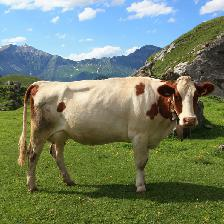
\includegraphics[width=\textwidth]{img/introduction/cow_original.jpg}
			\caption{Original}
		\end{subfigure}
		\hfill
		\begin{subfigure}[b]{0.22\textwidth}
			\centering
			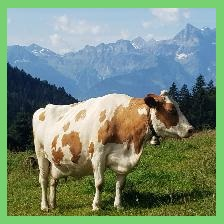
\includegraphics[width=\textwidth]{img/introduction/cow_noise.jpg}
			\caption{Sampling}
		\end{subfigure}
		\hfill
		\begin{subfigure}[b]{0.22\textwidth}
			\centering
			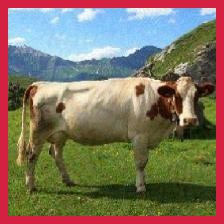
\includegraphics[width=\textwidth]{img/introduction/cow_fgsm.jpg}
			\caption{Adversarial}
		\end{subfigure}
		\hfill
		\begin{subfigure}[b]{0.22\textwidth}
			\centering
			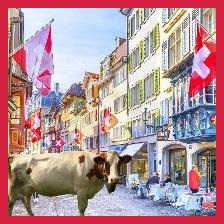
\includegraphics[width=\textwidth]{img/introduction/cow_ood.jpg}
			\caption{Distribution}
		\end{subfigure}
		   \caption{
			Illustrative example of the three expected sources of randomness in 
			the context of image classification. 
		   }
		   \label{fig:cows}
	\end{figure}
\end{frame}

% \begin{frame}{The robustness challenge -- Covariate shift}

% \end{frame}

\begin{frame}{The robustness challenge -- Challenges}
	\begin{itemize}
		\item Lack of understanding of the inductive bias.
		\item Robust vs non-robust features.
		\item Generalization-complexity trade-off.
	\end{itemize}

	\begin{figure}
		\centering
		\begin{subfigure}[t]{0.32\textwidth}
			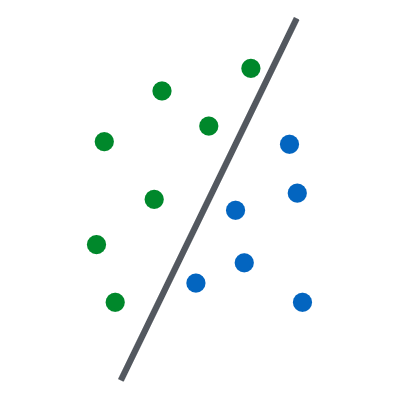
\includegraphics[width=0.6\textwidth]{img/introduction/adversarial_complexity_1.png}
			\caption{Linsep points}
		\end{subfigure}
		\hfill
		\begin{subfigure}[t]{0.32\textwidth}
			\centering
			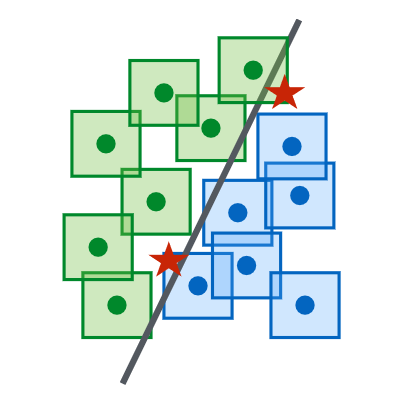
\includegraphics[width=0.6\textwidth]{img/introduction/adversarial_complexity_2.png}
			\caption{Standard training}
		\end{subfigure}
		\hfill
		\begin{subfigure}[t]{0.32\textwidth}
			\centering
			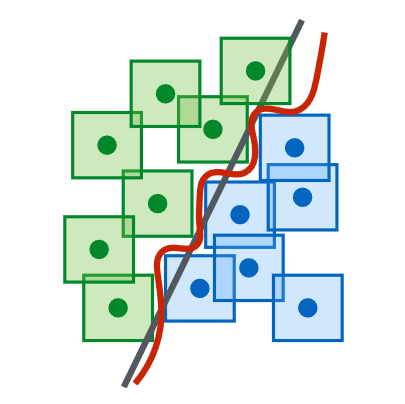
\includegraphics[width=0.6\textwidth]{img/introduction//adversarial_complexity_3.png}
			\caption{Adversarial training ($\ell_\infty$)}
		\end{subfigure}
		   \caption{
			Standard vs adversarial training decision boundaries. \cite{madryDeepLearningModels2019}
		   }
		   \label{fig:adversarial_complexity}
	\end{figure}
\end{frame}

\newsection{Learning framework}
\begin{frame}
    \centering
    \Huge{\insertsection}  % This will display the section title
\end{frame}

\begin{frame}{Learning framework -- Introduction}
	\textbf{Goal}: Learn a target function $f^*: \mathcal{X} \longmapsto \mathcal{Y}$ 
	by means of an approximated function $f \in \mathcal{F}$ using a 
	finite set of observations. 
	\vspace{0.5cm}

	\begin{itemize}
		\item Images $x \in \mathcal{X}$ belonging to $K = |\mathcal{Y}|$ classes.
		\item $f^*$ encodes the causal structure underlying the data generation process.
		\item $\mathcal{F}$ is composed of NN-parametrized classifiers.
	\end{itemize}
\end{frame}

% \begin{frame}{Learning framework -- Sampling experiment}
% 	\textbf{Definition} (\textit{Sample}): 
% 	\begin{itemize}
% 		\item Let $X$ be a random variable associated with a sampling 
% 		experiment in the input space, thus defining a measure of 
% 		probability $P_X$ with support $\mathcal{X}$.
% 		\item Let $\bm{X} = (X_1, ..., X_N)$ be a simple
% 		random sample of $X$ with size $N$. \\
% 	\end{itemize}
% 	A sample is a realization $\bm{x} \sim \bm{X}$.

% 	\vspace{0.5cm}
% 	A supervised dataset is constructed from $\bm{x}$ as:
% 	$$
% 	D = \{(x_n, f^*(x_n))\}_{n \in [N]}.
% 	$$
% \end{frame}

\begin{frame}{Learning framework -- Model}
	\textbf{Definition} (\textit{Classifier}): Let $K \in \mathbb{N} < \infty$ be the cardinality of $\mathcal{Y}$.
	$$
	\begin{aligned}
	f:\ & \mathcal{X} & \longmapsto & \quad \mathbb{R}^d & \longmapsto & \quad \mathbb{R}^K & \longmapsto & \quad \mathcal{Y} = \{1, \dots, K\} \\
		& x           & \longmapsto & \quad z & \longmapsto & \quad \bm{F}(z)    & \longmapsto & \quad \hat{y} = \arg \max_{k} F_k(z)
	\end{aligned}
	$$

	Under a NN parametrization $\Gamma$:


	$$
        \begin{aligned}
        f: \mathcal{X} \times \Gamma & \longmapsto \mathcal{Y} = \{1, \dots, K \} \\
        (x, \gamma) & \longmapsto f(x; \gamma) = \hat{y},
        \end{aligned}
    $$
\end{frame}


\begin{frame}{Learning framework -- Algorithm}
	\textbf{Definition} (\textit{K-class classification problem}):
	\begin{itemize}
		\item Let $L$ be the cross-entropy loss function.
		$$
		L(y) = - \log F_y(z; \gamma)
		$$
		\item Let $\hat{R}(f)$ be the empirical risk.
		$$
		\hat{R}(f)=\frac{1}{N}\sum_{n=1}^{N}L(f(x_{n}),f^{\star}(x_{n}))
		$$
	\end{itemize}

	$$
	\textcolor{black}{
        \boxed{
            \gamma^* = \arg \min_{\gamma \in \Gamma} - \frac{1}{N}\sum_{n=1}^{N} \log F_{y_n}(x_n; \gamma) + \lambda \Omega(\gamma)
        }
    }
	$$
\end{frame}

\newsection{Posterior Agreement}
\begin{frame}
    \centering
    \Huge{\insertsection}  % This will display the section title
\end{frame}

\begin{frame}{Posterior Agreement}
	\textbf{Definition} (\textit{Hypothesis class})
    A data science algorithm learns a function $f$ implementing the following mapping:

    $$
    \begin{aligned}
        f: \bm{X} & \longmapsto \Theta \\
        \bm{x}  & \longmapsto (f(x_1), \dots, f(x_N)) = \theta.
    \end{aligned}
    $$

	\textbf{Definition} (\textit{Posterior})
	The posterior $\mathbf{P}^f \in \mathfrak{P}^f$ establishes the stochastic relation between experiment realizations and hypotheses.
	$$
	\begin{aligned}
		\mathbf{P}^f: \bm{X} \times \Theta & \longmapsto \mathbb{R} \\
		(\bm{x}, \theta) & \longmapsto \mathbf{P}^f (\theta \mid \bm{x}).
	\end{aligned}
	$$
\end{frame}

\begin{frame}{Posterior Agreement}
	\textbf{Definition} (\textit{Generalization error}):
	\begin{itemize}
		\item Let $\bm{x'}$ and $\bm{x''}$ be realizations of $\bm{X}$.
		\item Let $\Theta$ be the hypothesis class represented by $f$ given $\bm{X}$. 
		\item Let $- \log \mathbf{P}^f (\cdot)$ be the description length of the posterior.
		
	\end{itemize}
		The generalization error is defined as the out-of-sample description length:
		$$
		\textcolor{black}{
        \boxed{
			\mathcal{G}_{\mathcal{X}} = \mathbb{E}_{\bm{x}', \bm{x}''} \mathbb{E}_{\mathbf{P}^f( \theta \mid \bm{x}')} \left[ - \log \frac{\mathbf{P}^f(\theta | \bm{x}'')}{\Pi^f (\theta)} \right].
			}
		}
		$$

		Intuitively, a low generalization error is obtained when good quality hypothesis
		on $\bm{x}''$ are likely to be drawn from $\bm{x}'$. 
\end{frame}

\begin{frame}
	\textbf{Lemma} (\textit{Posterior agreement}): The generalization error $\mathcal{G}_{\mathcal{X}}$ is non-negative and has a lower bound $-\mathcal{J}$. 
	$$
	\begin{aligned}
		\mathcal{G}_{\mathcal{X}} & \geq \mathbb{E}_{\bm{x}', \bm{x}''}\left[-\log \left(\mathbb{E}_{\mathbf{P}^f( \theta \mid \bm{x}')} \frac{\mathbf{P}^{f}\left(\theta \mid \bm{x}''\right)}{\Pi^{f}(\theta)}\right)\right] \\
		& = \textcolor{black}{\boxed{\mathbb{E}_{\bm{x}', \bm{x}''} \left[-\log \left(\sum_{\theta \in \Theta} \frac{\mathbf{P}^{f}\left(\theta \mid \bm{x}'\right) \mathbf{P}^{f}\left(\theta \mid \bm{x}'' \right)}{\Pi^{f}(\theta)}\right)\right] = -\mathcal{J}}} \\
		& \geq-\log \left(\mathbb{E}_{\bm{x}', \bm{x}''} \mathbb{E}_{\mathbf{P}^f( \theta \mid \bm{x}')} \mathbb{E}_{\mathbf{P}^f(\theta \mid \bm{x}'')} \frac{\mathbf{P}^{f}\left(\theta \mid \bm{x}''\right)}{\Pi^{f}(\theta)}\right)=0,
	\end{aligned}
	$$
	
	where Jensen's inequality has been applied twice to the convex function $-\log$. \\
\end{frame}

\begin{frame}
	\textbf{Proposition}: Posterior agreement based model selection criterion.

    $$
    \begin{aligned}
        \sup_{\mathcal{F}} & \; \mathcal{J} \\
        \text{s.t.} & \; \text{KL}(\mathbf{\Pi}^f(\theta) \parallel |\Theta|^{-1}) \leq \xi,
    \end{aligned}
    $$
    where $\xi \in \mathbb{R}$ represents a small allowed deviation from uniformity in the prior.

	\vspace{0.5cm}

	\textbf{Theorem} (\textit{Maximum posterior agreement}): The optimal $\mathbf{P}_{*}^f$ maximizing the posterior 
	agreement criterion defines a lower bound in the generalization error $\mathcal{G}_{\mathcal{X}}$:
		
	$$
		\inf_{\mathcal{F}} \mathcal{G}_{\mathcal{X}} \geq -\sup_{\mathcal{F}} \mathcal{J}.
	$$
\end{frame}

\begin{frame}
    \textbf{Proposition} (\textit{Posterior Agreement kernel}): With no prior information about $\Theta$, the posterior agreement kernel
    for supervised $K$-class classification tasks has the following expression:

    $$
    \textcolor{blue}{
        \boxed{
            \operatorname{PA}\left(\bm{x}', \bm{x}'' ; \beta\right)=\frac{1}{N} \sum_{n=1}^N \log \left\{|\Theta| \sum_{k= 1}^K \mathbf{P}^c\left(k \mid x_n' \right) \mathbf{P}^c \left( k \mid x_n'' \right)\right\},
        }
    }
    $$

	\vspace{0.5cm}

    where $\mathbf{P}^c(j \mid x_n)$ can be shown to be

    $$
    \textcolor{blue}{
        \boxed{
            \mathbf{P}^c\left(k \mid x_n\right)=\frac{\exp\left(\beta F_{k}(x_n)\right)}{\sum_{q=1}^K\exp\left(\beta F_q(x_n)\right)}.
        }
    }
    $$
\end{frame}


\begin{frame}
	\textbf{Theorem.} The posterior agreement kernel for $K$-classification 
	problems $\operatorname{PA}\left(\bm{x}', \bm{x}'' ; \beta\right)$ has the following 
	properties $\forall \bm{x}', \bm{x}'' \sim \bm{X}$ and $\beta \in \mathbb{R}^+$.

	\vspace{0.15cm}

    \begin{itemize}
        \item[P1](Boundedness) $\operatorname{PA}\left(\bm{x}', \bm{x}'' ; \beta\right) \leq N \log{K}$. Because $\log_2 K$ bits are 
		needed to encode a uniform distribution over the classes for each observation.
        \item[P2](Symmetry)  $\operatorname{PA}\left(\bm{x}', \bm{x}'' ; \beta\right) = \operatorname{PA}\left(\bm{x}'', \bm{x}'; \beta\right)$. 
		Because randomness instantiations are not observable.
        \item[P3](Concavity) $\operatorname{PA}\left(\bm{x}', \bm{x}'' ; \beta\right)$ is a concave function of $\beta \in \mathbb{R}^+$. 
		Then the kernel optimization problem will have a unique solution.
    \end{itemize}

	\vspace{0.5cm}
	
	In particular, the maximum value  $\operatorname{PA} \equiv \operatorname{PA}\left(\bm{x}', \bm{x}'' ; \beta^{*} \right)$ is bounded by
	the situations $\beta^{*} \longrightarrow 0$ and $\beta^{*} \longrightarrow \infty$. Then:
	$$
    -N \log K \leq \operatorname{PA} \leq 0
    $$


	
\end{frame}

\begin{frame}
	\begin{figure}[H]
		\centering
		\begin{subfigure}[b]{0.9\textwidth}
			\begin{subfigure}[b]{0.3\textwidth}
				\centering
				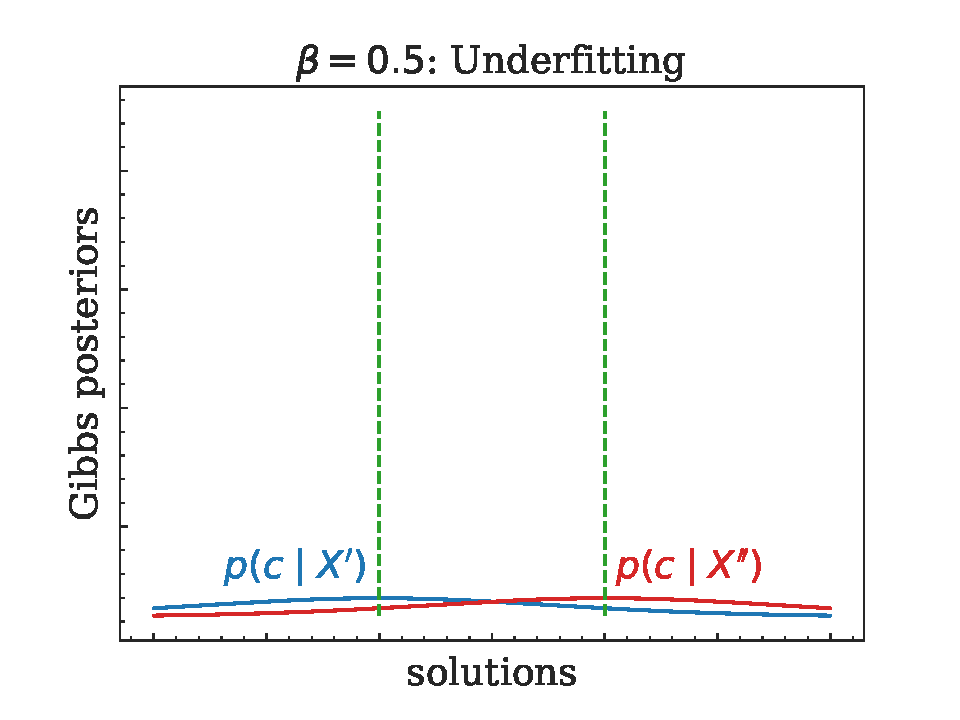
\includegraphics[width=\textwidth]{img/theoretical_background/method_beta=0.5.pdf}
			\end{subfigure}
			\hfill
			\begin{subfigure}[b]{0.3\textwidth}
				\centering
				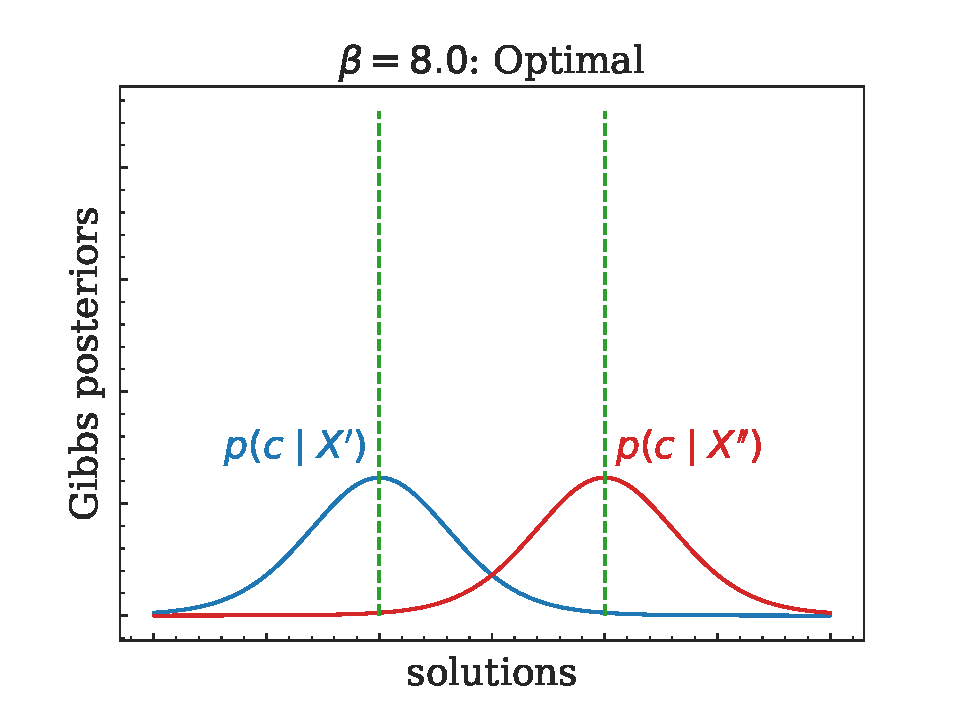
\includegraphics[width=\textwidth]{img/theoretical_background/method_beta=8.0.pdf}
			\end{subfigure}
			\hfill
			\begin{subfigure}[b]{0.3\textwidth}
				\centering
				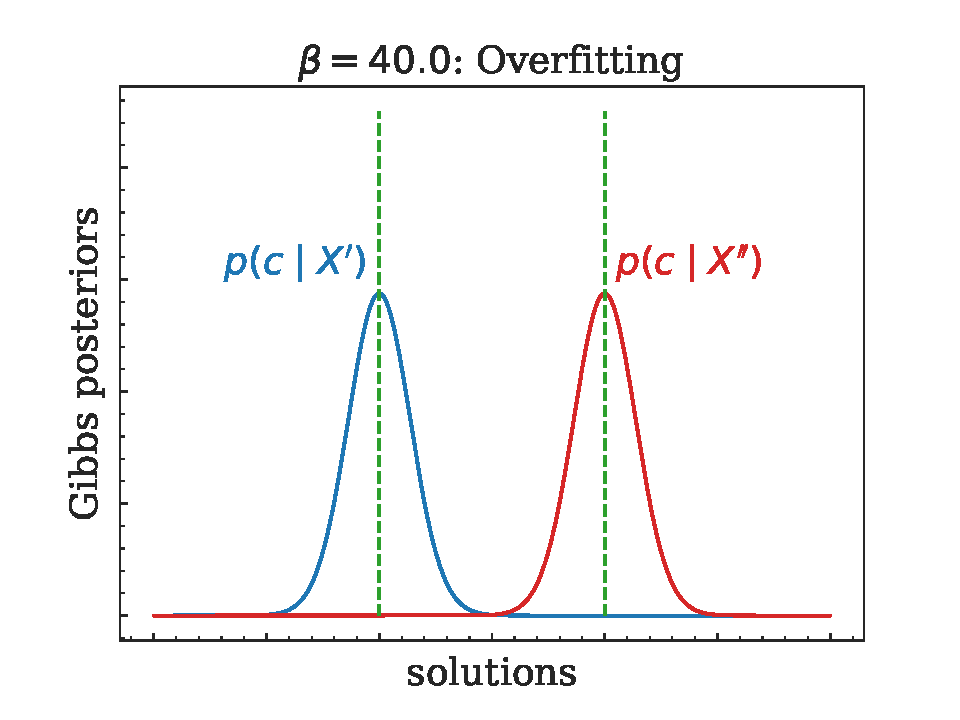
\includegraphics[width=\textwidth]{img/theoretical_background/method_beta=40.0.pdf}
			\end{subfigure}
		
			\vspace{1em}
		
			\begin{subfigure}[b]{0.975\textwidth}
				\hspace{0.05cm}
				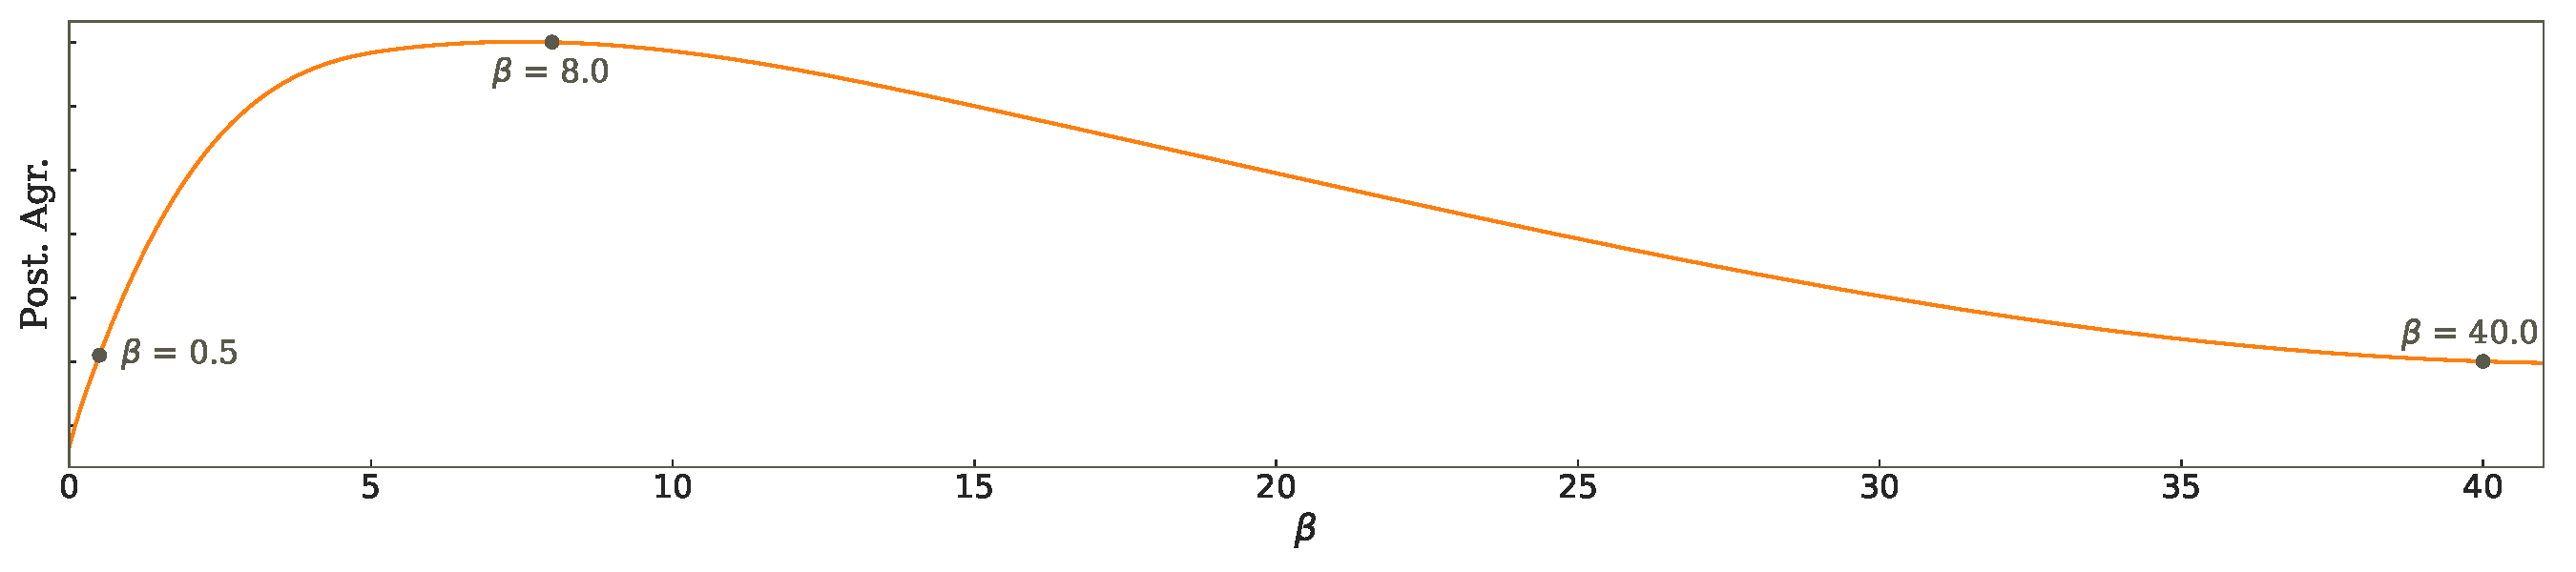
\includegraphics[width=\textwidth]{img/theoretical_background/gibbs_betas.pdf}
			\end{subfigure}
		\end{subfigure}
		
		\caption{
			Illustration of the optimization over the inverse temperature parameter $\beta$. 
			Posterior Agreement is maximum at a value $\beta^{*}$ 
			in which hypothesis selected from the posterior over $\theta \mid \bm{x^\prime}$ are assigned
			a high probability by the posterior over $\theta \mid \bm{x^{\prime\prime}}$.
		}
	\end{figure}
\end{frame}


\newsection{Robustness against covariate shift}
\begin{frame}
    \centering
    \Huge{\insertsection}  % This will display the section title
\end{frame}

% \begin{frame}{Robustness against covariate shift -- Covariate shift}
% 	\textbf{Definition} (\emph{Covariate shift}): Let $\bm{x}'$ and $\bm{x}''$ be two samples of $\bm{X} \overset{\text{iid}}{\sim} X$.
% 		$$
% 		\mathbf{P}_{\bm{x}'} \not \sim \mathbf{P}_{\bm{x}''}.
% 		$$
		
% 	\textbf{Definition} (\emph{Distribution shift}): Let $X'$ and $X''$ be two random variables associated to different sampling 
%     experiments in $\mathcal{X}$ such that $P_{X'} \not \sim P_{X''}$.
% 	$$
%         \bm{x}' \sim \bm{X}' \overset{\text{iid}}{\sim} X' \text{ and } \bm{x}'' \sim \bm{X}'' \overset{\text{iid}}{\sim} X''
%     $$
% 	% Then, $X' \neq X'' \Longrightarrow \mathbf{P}_{\bm{x}'} \not \sim \mathbf{P}_{\bm{x}''}$ in general.

% 	\textbf{Definition} (\emph{Adversarial shift}): Let $\bm{x}' \sim \bm{X}$ be a sample drawn from experiment
%     $X$. Let $\bm{\Delta}$ be a perturbation over
%     the sample space.

%     $$
%     \bm{x}'' = \bm{x}' + \bm{\Delta},
%     $$
% \end{frame}


\begin{frame}{Robustness against covariate shift -- Robustness metric}
	\textbf{Proposition.} A robustness metric should possess the following properties:
	\begin{itemize}
		\item[P1](Non-increasing) The metric should be non-increasing with respect to the
		response of the model under increasing levels of covariate shift.
		\item[P2](Independent discriminability) The metric should discriminate models exclusively by their generalization capabilities against 
		covariate shift. For instance, the metric should be independent of the task
		performance.
	\end{itemize}

	\vspace{0.5cm}

	% \textbf{Example} Consider the following classifiers:
	% \begin{itemize}
	% 	\item Perfect classifier: High performance, high robustness.
	% 	\item Constant classifier: Low performance, high robustness.
	% 	\item Random classifier: Low performance, low robustness.
	% \end{itemize}

	\textbf{Example I.} Consider the following classifiers in a balanced dataset:
	\begin{table}[H]
		\centering
		\begin{tabular}{l|c|l}
		Classifier & Performance & Robustness \\
		\midrule
		Perfect   & 1.0  & Max.  \\
		Constant  & $1/K$  & Max.   \\
		Random    & $1/K$   & Min.   \\
		\bottomrule
		\end{tabular}
	\end{table}

\end{frame}

\begin{frame}
	A binary sample $\bm{y} \overset{\text{iid}}{\sim} \operatorname{Bernoulli}(p)$ of size 1000 is generated, 
    with $p = \mathbf{P}_Y(y = 1)$. 

	\begin{itemize}
        \item For a perfect classifier, predictions are $\hat{\bm{y}}^\prime = \hat{\bm{y}}^{\prime \prime} = \bm{y}$.
        \item For a constant classifier, predictions are $\hat{\bm{y}}^\prime = \hat{\bm{y}}^{\prime \prime} = \bm{0}$.
        \item For a random classifier, predictions $\hat{\bm{y}}^\prime, \hat{\bm{y}}^{\prime \prime}$ are generated by randomly permuting $\bm{y}$, so 
        that the number of mismatched observations depends on the value of $p$. 

        % $$
        %     \hat{\bm{y}}^\prime, \hat{\bm{y}}^{\prime \prime} \sim \operatorname{Permutation}(\bm{y})
        % $$
    \end{itemize}

	\begin{figure}[t]
		\centering
		\begin{subfigure}[b]{0.35\textwidth}
			\centering
			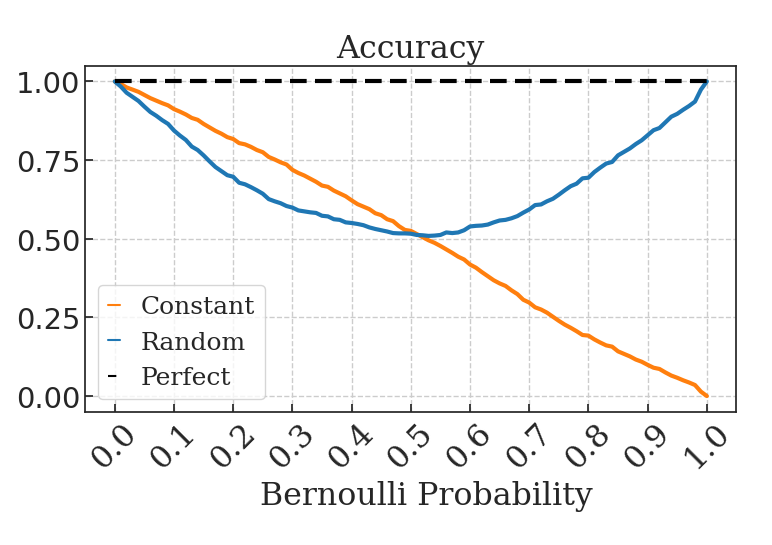
\includegraphics[width=\textwidth]{img/experimental_setup/artificial_acc_final.png}
		\end{subfigure}
		\hspace{1em}
		\begin{subfigure}[b]{0.35\textwidth}
			\centering
			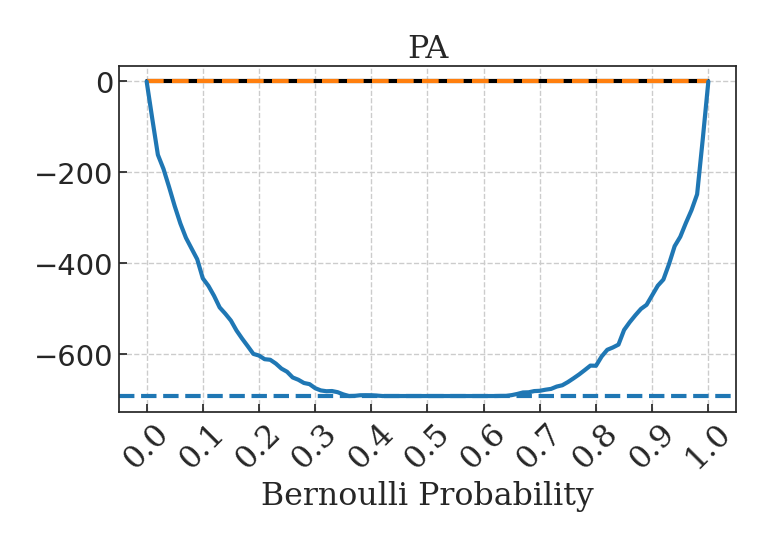
\includegraphics[width=\textwidth]{img/experimental_setup/artificial_logPA_final.png}
		\end{subfigure}
		\caption{
		Evolution of PA and accuracy for constant, perfect and random classifiers across different 
		values of $p \in [0,1]$.
		}
		\label{fig:empirical_plot}
	\end{figure}
\end{frame}

\begin{frame}
	\textbf{Example II.} Consider a sentiment classifier in the IMDB dataset. $\bm{x}^\prime$ is a sample of original
	reviews, and $\bm{x}^{\prime\prime}$ is formed by manipulating every $x \in \bm{x}^\prime$.

	\begin{itemize}
		\item Levenshtein: Addition, removal or substitution of characters.
		\item Amplification: Addition of reinforcing adjectives.
		\item Contradiction: Addition of contradicting adjectives.
	\end{itemize}

	\begin{figure}[H]
		\centering
		\begin{subfigure}[b]{0.3\textwidth}
			\centering
			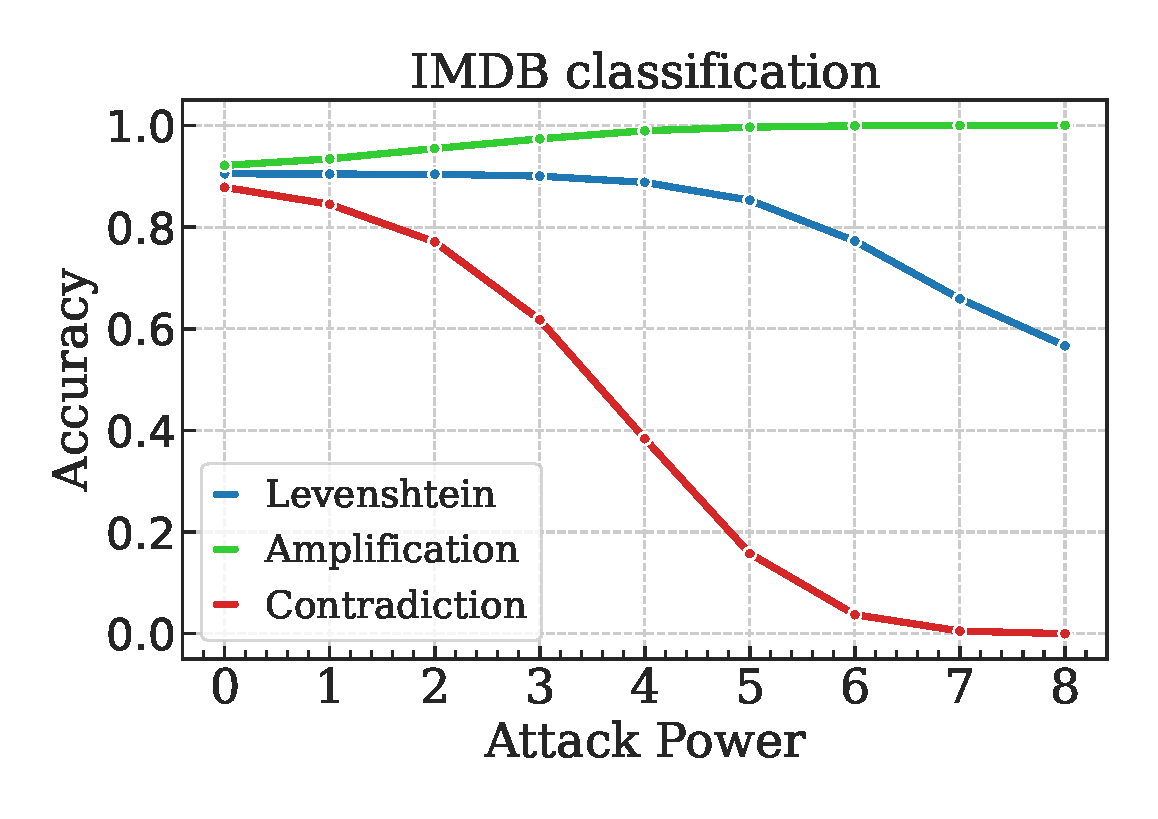
\includegraphics[width=\textwidth]{img/experimental_setup/presentation_acc.pdf}
		\end{subfigure}
		\hspace{1em}
		\begin{subfigure}[b]{0.3\textwidth}
			\centering
			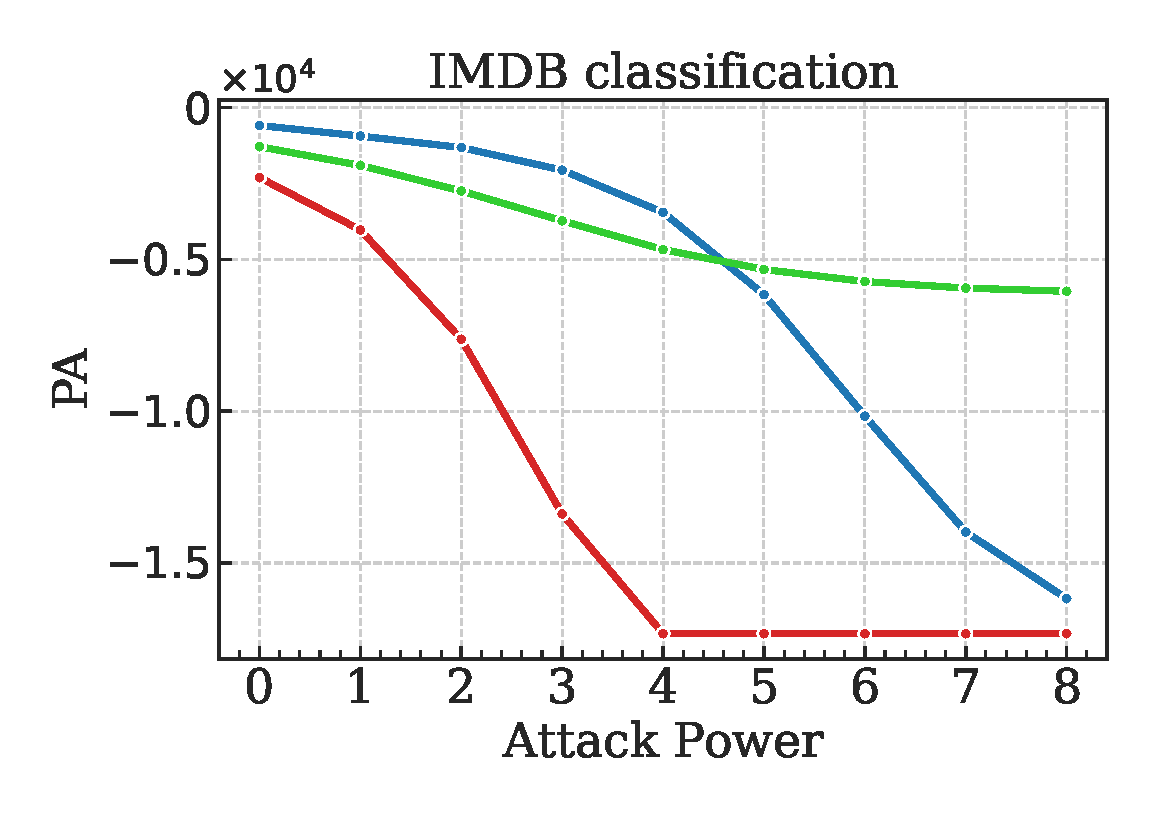
\includegraphics[width=\textwidth]{img/experimental_setup/presentation_pa.pdf}
		\end{subfigure}
		\caption{
			Accuracy and PA for the IMDB sentiment classification task under random 
			and adversarial perturbations. The attack power is defined as $2^W$, being $W$ the
			number of modifications performed.
		}
	\end{figure}
\end{frame}

\newsection{Adversarial setting}
\begin{frame}
    \centering
    \Huge{\insertsection}  % This will display the section title
\end{frame}


\begin{frame}{Adversarial setting -- Attacks}
	\textbf{Definition} (\textit{Perturbation}) Let $\mathbf{B}_p^\epsilon(x)$ be the $\ell_p$-norm ball of radius 
		$\epsilon$ centered at observation $x$. A perturbation $\Delta$ is defined as
	
		$$
			\Delta \in \mathbb{R}^d \text{ s.t. } x + \Delta \in \mathbf{B}_p^\epsilon(x),
		$$

	\textbf{Attack} (\textit{PGD}): Projected gradient descent.
	$$
        x^{s+1} = \Pi_{\mathbf{B}_p^\epsilon(x)} \left ( x^s + \Delta \right ); \quad \Delta = \epsilon_p \operatorname{sign}(\nabla_{x'} \mathcal{L}(x', y; \gamma))
    $$

	\textbf{Attack} (\textit{FMN}): Fast minimum norm.
	$$
        \begin{aligned}
            \Delta^\star = \arg \min_\Delta & \; ||\Delta||_p \\
            \text { s.t. } & F_y(x; \gamma)- \max_{k \neq y} F_k(x; \gamma) < 0, \\
            & x + \Delta \in \mathbf{B}_p^\epsilon(x).
        \end{aligned}
    $$
\end{frame}

\begin{frame}{Adversarial setting -- Characterization}
	\textbf{Definition} (\textit{Adversarial ratio}) Measures the ratio of perturbed observations in the dataset, 
    also known as adversarial ratio $\alpha \in [0,1]$. The final adversarial dataset $\bm{x}''$ will be generated as

    $$
    \bm{x}'' := \alpha \bm{x}'' + (1 - \alpha) \bm{x}', \quad \bm{x}'' = \bm{x}' + \bm{\Delta}
    $$

	\textbf{Definition} (\textit{Attack failure rate}) 
	Let $\hat{\bm{y}}^\prime, \hat{\bm{y}}^{\prime\prime} \in \mathcal{Y}^N$ be the predicted class 
    labels for $\bm{x}^\prime$ and $\bm{x}^{\prime \prime}$, respectively, 
    and let $\bm{y}\in \mathcal{Y}^N$ be the true labels.

	$$
        \operatorname{AFR}_\text{T} = \operatorname{Accuracy}(\hat{\bm{y}}^{\prime \prime}, \bm{y}), \quad
        \operatorname{AFR}_\text{P} = \operatorname{Accuracy}(\hat{\bm{y}}^{\prime \prime}, \hat{\bm{y}}^{\prime}).
    $$

	\vspace{0.2cm}

	The variation of $\operatorname{AFR}$ with respect to $\alpha$ is also reported:

	$$
		\Delta \operatorname{AFR} = \operatorname{AFR}_\text{T}\biggr|_{\alpha = 1} - \operatorname{AFR}_\text{T}\biggr|_{\alpha = 0} = \operatorname{AFR}_\text{P}\biggr|_{\alpha = 1} - \operatorname{AFR}_\text{P}\biggr|_{\alpha = 0}
	$$

\end{frame}

\begin{frame}{Adversarial setting -- Experimental setup}
		\textbf{Experimental setup. }{\small \color{black} CIFAR10 \cite{krizhevskyLearningMultipleLayers} is
		a balanced dataset containing 60.000 colored 32 $\times$ 32 pixel images belonging to 10
		different classes. We will consider a pre-trained WideResNet-28-10
		\cite{BMVC2016_87}
		as a baseline, {\color{tab:orange} \textbf{Undefended}} model and compare it to some state-of-the-art robust ResNet50
		\cite{resnet50}
		models provided by the 
		RobustBench \cite{croceRobustBenchStandardizedAdversarial2021a}
		library under PGD \cite{madryDeepLearningModels2019}
		and FMN \cite{pintorFastMinimumnormAdversarial2021}
		attacks, both run for 1000 steps.
		The defenses applied are those proposed by 
		{\color{tab:blue} \textbf{Engstrom et al.}} \cite{engstrom2019adversarial}, 
		{\color{tab:green} \textbf{Athalye et al.}} \cite{AthalyeC018}, 
		{\color{tab:red} \textbf{Wong et al.}} \cite{WongRK20}, 
		{\color{tab:purple} \textbf{Addepalli et al.}} \cite{Addepalli2022ScalingAT}
		and {\color{tab:brown} \textbf{Wang et al.}} \cite{wang2023betterdiffusionmodelsimprove}.
		}
		
		\vspace{0.2cm}

		\begin{figure}[H]
			\centering
			\begin{subfigure}[t]{0.3\textwidth}
				\centering
				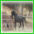
\includegraphics[width=0.5\textwidth]{img/adversarial/adv_unperturbed_framed.png}
				\caption{Original}
			\end{subfigure}
			\hspace{1em}
			\begin{subfigure}[t]{0.3\textwidth}
				\centering
				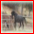
\includegraphics[width=0.5\textwidth]{img/adversarial/adv_pgd_framed.png}
				\caption{PGD, $\ell_\infty$ = 36/255}
			\end{subfigure}
			\hspace{1em}
			\begin{subfigure}[t]{0.3\textwidth}
				\centering
				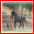
\includegraphics[width=0.5\textwidth]{img/adversarial/adv_fmn_framed.png}
				\caption{FMN}
			\end{subfigure}
			\caption{Original and adversarially-perturbed CIFAR10 observation of class \texttt{horse}.}
		\end{figure}
\end{frame}

\begin{frame}{Adversarial setting -- PGD}
	\textbf{Experiment 1.}
	A pre-trained, undefended WideResNet-28-10 and five RobustBench
	defended models are subject to a 1000 step PGD attack with $\ell_\infty = 8/255$.

	\begin{figure}[H]
		\centering
		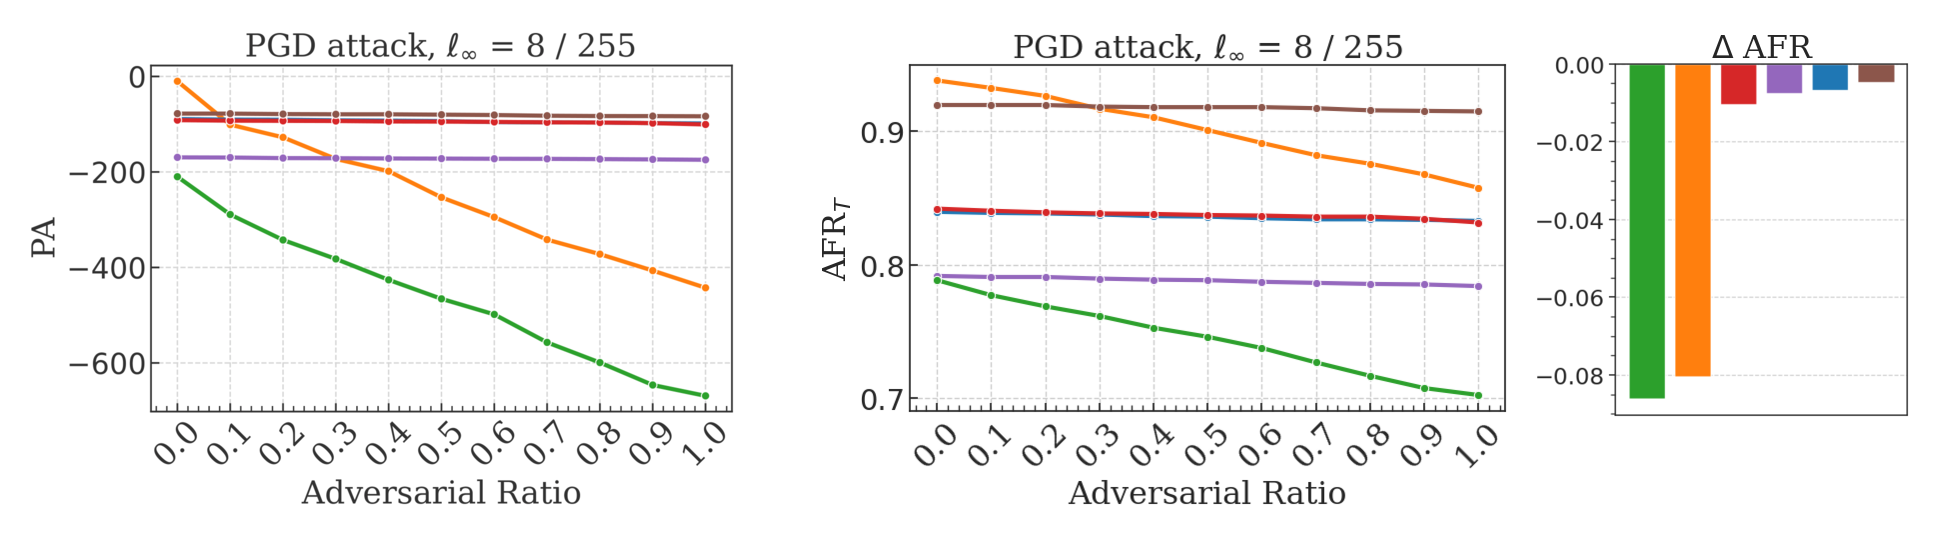
\includegraphics[width=\textwidth]{img/adversarial/PGD_0.0314_combo2.png}
		\caption{
		PA, $\operatorname{AFR}_\text{T}$ and the AFR variation against increasing 
		adversarial ratio $\alpha \in [0,1]$.
		}
		\label{fig:six_figures_pa_adv}
	\end{figure}
\end{frame}

\begin{frame}{Adversarial setting -- PGD}

	\begin{figure}[H]
		\centering
		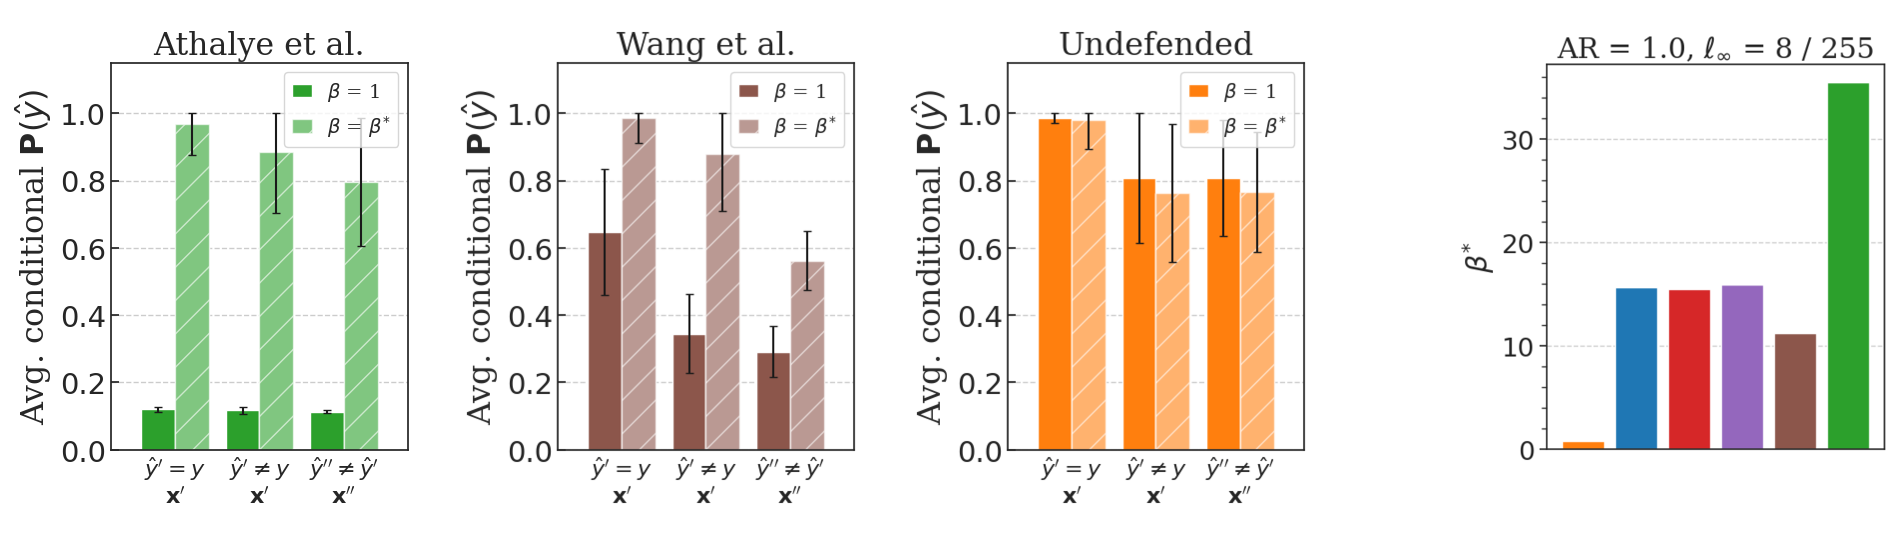
\includegraphics[width=\textwidth]{img/adversarial/bpda_wang_undefended_beta_pgd.png}
		\caption{
			(\textbf{left}) Average posterior probability of the predicted class for 
			correctly classified original observations, misclassified original observations and 
			misleading adversarial observations. (\textbf{right}) Optimal $\beta^{*}$ value achieved by each 
			model.
		}
		\label{fig:six_figures_pa_adv}
	\end{figure}
\end{frame}

% \begin{frame}{Adversarial setting -- FMN}
% 	\textbf{Experiment 2.}
% 	A pre-trained, undefended WideResNet-28-10 and five RobustBench
% 	defended models are subject to a 1000 step FMN attack.

% 	\begin{figure}[H]
% 		\centering
% 		\begin{subfigure}[b]{0.39\textwidth}
% 			\centering
% 			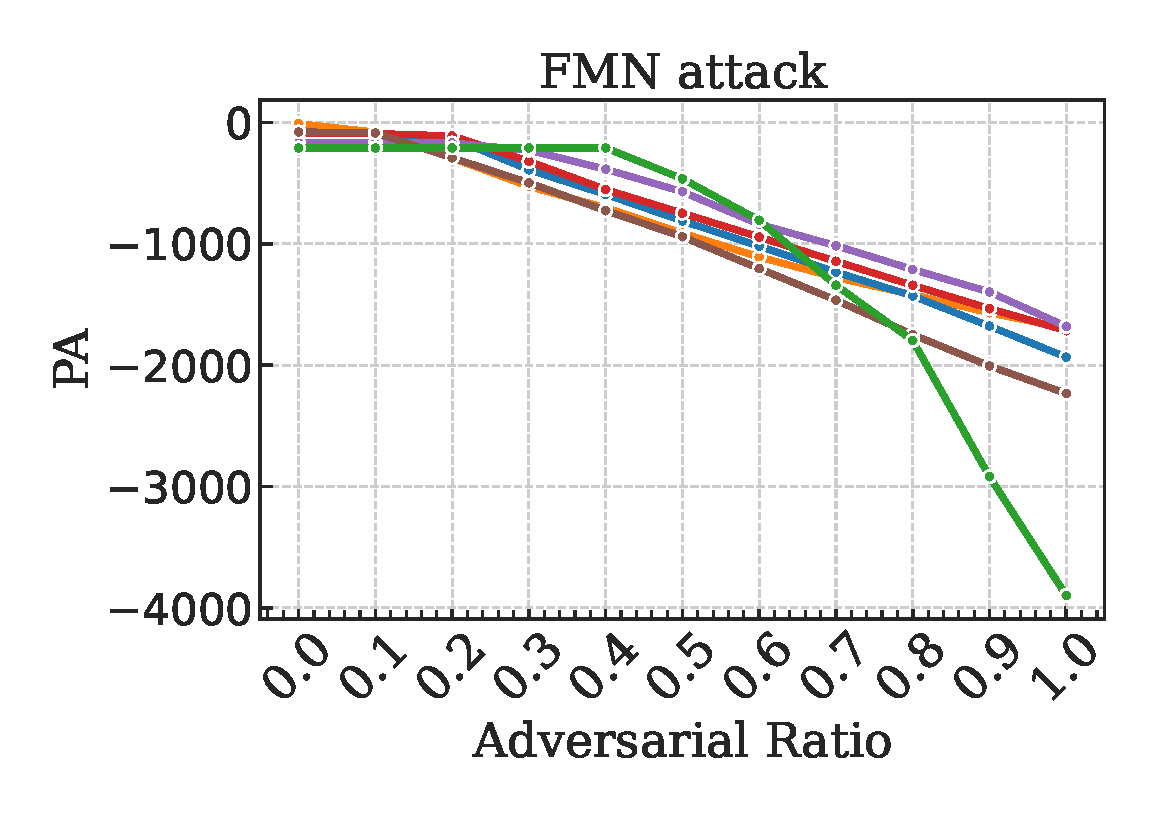
\includegraphics[width=\textwidth]{img/adversarial/FMN_1000_logPA.pdf}
% 		\end{subfigure}
% 		\hfill
% 		\begin{subfigure}[b]{0.59\textwidth}
% 			\centering
% 			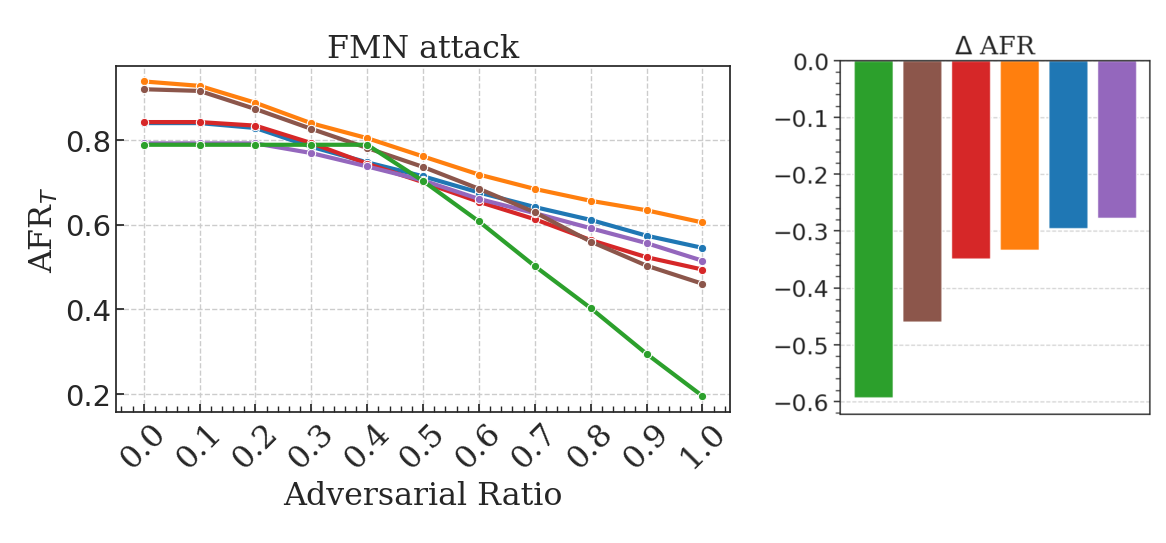
\includegraphics[width=\textwidth]{img/adversarial/FMN_1000_AFR_true.png}
% 		\end{subfigure}
% 		\caption{PA, $\operatorname{AFR}_\text{T}$ and the AFR variation against increasing adversarial ratio. 
% 		The undefended net and several RobustBench robust models are considered 
% 		under a 1000 step FMN attack.}
% 		\label{fig:adv_fmn_pa_afr}
% 	\end{figure}
% \end{frame}

\begin{frame}{Adversarial setting -- FMN}
	\begin{figure}[H]
		\centering
		\begin{subfigure}[b]{\textwidth}
			\centering
			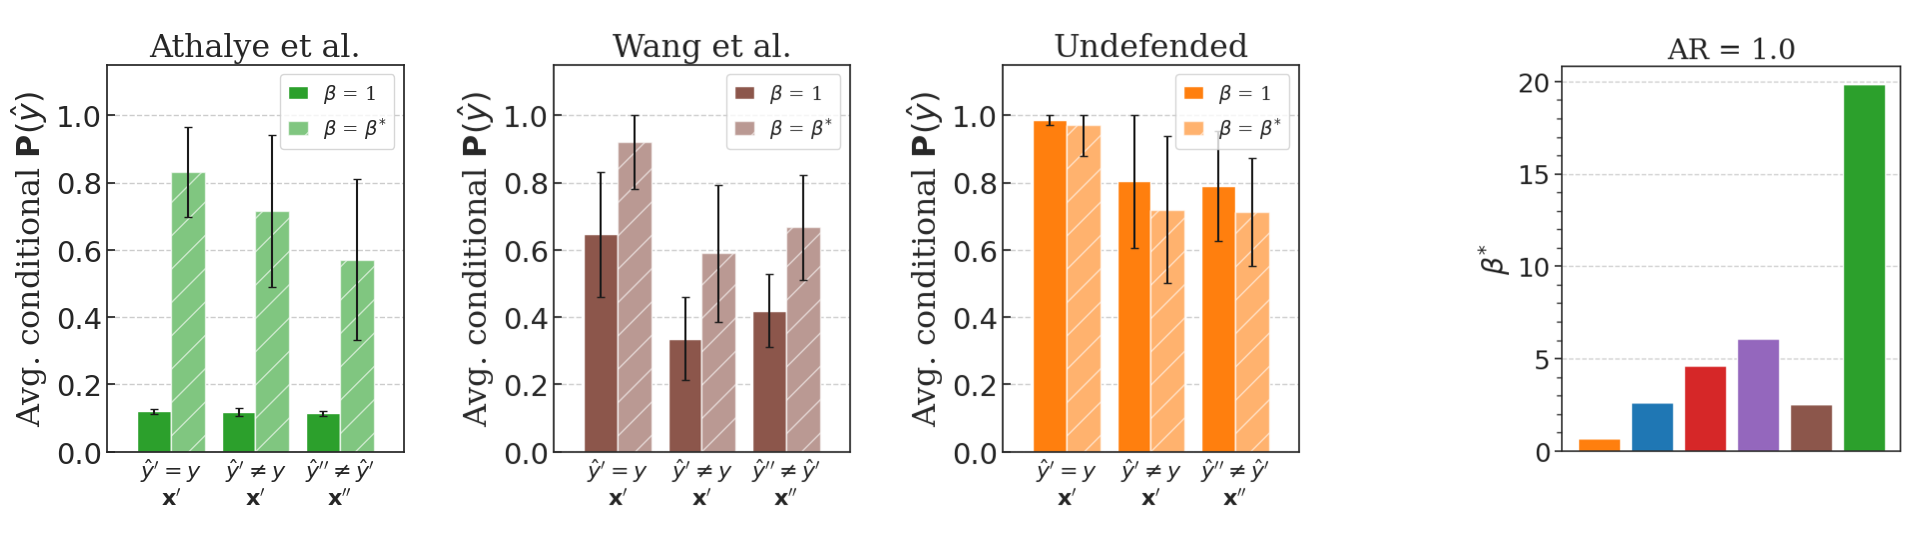
\includegraphics[width=\textwidth]{img/adversarial/bpda_wang_undefended_beta_fmn.png}
		\end{subfigure}
	   
		\caption{(\textbf{left}) Average posterior probability of the predicted class under
		FMN attack for correctly classified original observations, misclassified original observations, and 
		misleading adversarial observations.
		(\textbf{right}) Optimal $\beta^{*}$ value for each model.
		}
		\label{fig:unrobust_posterior_short_fmn}
	\end{figure}
\end{frame}

\begin{frame}{Adversarial setting -- PGD vs FMN}

	\textbf{Comparison between metrics.}
	
\begin{table}[h]
    \centering
    \resizebox{0.8\textwidth}{!}{%
    \begin{tabular}{l|ccc|ccc|ccc}
    \multirow{2}{*}{} & \multicolumn{3}{c|}{$\alpha$ = 2/10} & \multicolumn{3}{c|}{$\alpha$ = 4/10} & \multicolumn{3}{c}{$\alpha$ = 6/10} \\
    % \cmidrule{2-10}
    \textbf{PGD} & PA & $\operatorname{AFR}_{\text{P}}$ & $\operatorname{AFR}_{\text{T}}$ & PA & $\operatorname{AFR}_{\text{P}}$  & $\operatorname{AFR}_{\text{T}}$ & PA & $\operatorname{AFR}_{\text{P}}$  & $\operatorname{AFR}_{\text{T}}$ \\
    \midrule
    {\color{tab:purple} \textbf{Addepalli et al.}} & \textbf{-172.5} & \textbf{0.995} & \textbf{0.785} & \textbf{-175.5} & 0.992  & \textbf{0.786} & \textbf{-177.6} & 0.989  & \textbf{0.783} \\
    {\color{tab:red} \textbf{Wong et al.}} & -97.7 & 0.996  & 0.838 & -102.9 & 0.992  & 0.834 & -109.2 & \textbf{0.987}  & 0.830 \\
    {\color{tab:blue} \textbf{Engstrom et al.}} & -94.2 & 0.996 & 0.836 & -104.6 & \textbf{0.990} & 0.830 & -110.3 & 0.988 & 0.829 \\
    {\color{tab:brown} \textbf{Wang et al.}} & -81.9 & 0.997 & 0.917 & -84.6 & 0.996 & 0.915 & -89.4 & 0.991 & 0.912 \\
    \midrule
    \addlinespace
    \addlinespace
    \textbf{FMN} & PA & $\operatorname{AFR}_{\text{P}}$ & $\operatorname{AFR}_{\text{T}}$ & PA & $\operatorname{AFR}_{\text{P}}$  & $\operatorname{AFR}_{\text{T}}$ & PA & $\operatorname{AFR}_{\text{P}}$  & $\operatorname{AFR}_{\text{T}}$ \\
    \midrule
    {\color{tab:purple} \textbf{Addepalli et al.}} & -169.4 & 1.0 & \textbf{0.791} & -385.4 & 0.944  & \textbf{0.737} & --838.9 & 0.867  & 0.660 \\
    {\color{tab:red} \textbf{Wong et al.}} & -111.2 & 0.991  & 0.834 & -553.1 & 0.901  & 0.743 & -944.8 & 0.810  & \textbf{0.653} \\
    {\color{tab:blue} \textbf{Engstrom et al.}} & -128.5 & 0.988 & 0.828 & -592.9 & 0.907 & 0.747 & -1020 & 0.836 & 0.675 \\
    {\color{tab:brown} \textbf{Wang et al.}} & \textbf{-291.6} & \textbf{0.952} & 0.873 & \textbf{-726.8} & \textbf{0.861} & 0.781 & \textbf{-1204} & \textbf{0.764} & 0.684 \\
    \bottomrule
    \end{tabular}%
    }
    \caption{
        Comparison of PA, $\operatorname{AFR}_{\text{P}}$ and $\operatorname{AFR}_{\text{T}}$ scores for a 
        PGD attack with $\ell_\infty$=16/255 and a FMN attack across different adversarial 
        ratio values.
    }
    \label{tab:pa_afrpred_comparison_table}
\end{table}
\end{frame}

\begin{frame}{Adversarial setting -- PGD vs FMN}
	\textbf{Approximated PA contributions.} A surrogate version of the PA kernel can be obtained considering the average posterior
	for the two main robustness contributions:
	\begin{itemize}
		\item Sampling randomness contribution $\zeta_{\text{SAM}}$, accounting for $N_{\text{SAM}}$ misclassified observations in $\bm{x}^\prime$
		with average probability $\rho_{\text{MIS}}$.
		\item Adversarial attack contribution $\zeta_{\text{ADV}}$, accounting for $N_{\text{ADV}}$ misleading adversarial observations in $\bm{x}^{\prime \prime}$
		with average probability $\rho_{\text{ADV}}$.
	\end{itemize}
	\begin{table}[H]
		\centering
		\resizebox{0.9\textwidth}{!}{%
		\begin{tabular}{l|rrr|rrr||rrr|rrr}
		\multirow{2}{*}{} & \multicolumn{6}{c||}{\textbf{PGD}, $\ell_\infty$=16/255} & \multicolumn{6}{c}{\textbf{FMN}} \\
		Defense & $N_{\text{MIS}}$ & $\rho_{\text{MIS}}$ & \textbf{$\zeta_{\text{SAM}}$} & $N_{\text{ADV}}$ & $\rho_{\text{ADV}}$ & \textbf{$\zeta_{\text{ADV}}$} & $N_{\text{MIS}}$ & $\rho_{\text{MIS}}$ & \textbf{$\zeta_{\text{SAM}}$} & $N_{\text{ADV}}$ & $\rho_{\text{ADV}}$ & \textbf{$\zeta_{\text{ADV}}$} \\
		\midrule
		{\color{tab:brown} \textbf{Wang et al.}} & 799 & 0.88 & \textbf{-468.62} & 47 & 0.56 & \textbf{-39.44} & 435 & 0.59 & \textbf{-1599.08} & 4215 & 0.67 & \textbf{-4637.45} \\
		{\color{tab:blue} \textbf{Engstrom et al.}} & 1591 & 0.91 & \textbf{-566.72} & 67 & 0.61 & \textbf{-63.43} & 1125 & 0.64 & \textbf{-2469.65} & 2505 & 0.68 & \textbf{-2847.99} \\
		{\color{tab:red} \textbf{Wong et al.}} & 1562 & 0.91 & \textbf{-537.25} & 90 & 0.62 & \textbf{-88.98} & 1032 & 0.77 & \textbf{-1125.53} & 2920 & 0.73 & \textbf{-3844.40} \\
		{\color{tab:purple} \textbf{Addepalli et al.}} & 2063 & 0.89 & \textbf{-877.42} & 75 & 0.54 & \textbf{-58.92} & 1507 & 0.74 & \textbf{-1910.69} & 2187 & 0.72 & \textbf{-2788.89} \\
		\midrule
		{\color{tab:orange} \textbf{Undefended}} & 566 & 0.77 & \textbf{-736.63} & 810 & 0.76 & \textbf{-1173.55} & 412 & 0.72 & \textbf{-704.58} & 3132 & 0.71 & \textbf{-3906.55} \\
		{\color{tab:green} \textbf{Athalye et al.}} & 1915 & 0.88 & \textbf{-963.85} & 747 & 0.79 & \textbf{-1183.96} & 859 & 0.74 & \textbf{-2054.23} & 4679 & 0.57 & \textbf{-3955.43} \\
		\bottomrule
		\end{tabular}
		}
		\caption{
		Approximated PA contributions for a PGD attack with $\ell_\infty$=16/255 and a FMM attack.
		}
	\end{table}

\end{frame}


\newsection{Out-of-distribution setting}
\begin{frame}
    \centering
    \Huge{\insertsection}  % This will display the section title
\end{frame}

\begin{frame}{Out-of-distribution setting -- Robust learners}
	\begin{itemize}
		\item \textbf{IRM} (domain alignment): Regularization term that pushes towards the minimization of the dissimilarity of
		feature representations originated from different source environments \cite{arjovskyInvariantRiskMinimization2020}.
		\item \textbf{LISA} (data augmentation): Artificial observations are generated by intra-domain and/or intra-label
		interpolation \cite{yaoImprovingOutofDistributionRobustness2022}.
	\end{itemize}

	\begin{figure}[H]
		\centering
		\begin{subfigure}[t]{0.3\textwidth}
			\centering
			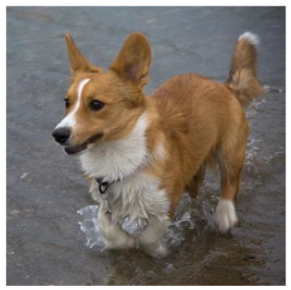
\includegraphics[width=0.5\textwidth]{img/distribution/da_original.png}
			\caption{Original}
		\end{subfigure}
		\hspace{0.65em}
		\begin{subfigure}[t]{0.3\textwidth}
			\centering
			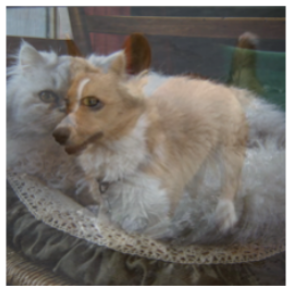
\includegraphics[width=0.5\textwidth]{img/distribution/da_mixup.png}
			\caption{Mixup 
			\cite{zhangMixupEmpiricalRisk2018}
			}
		\end{subfigure}
		\hspace{0.65em}
		\begin{subfigure}[t]{0.3\textwidth}
			\centering
			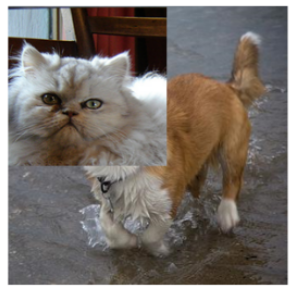
\includegraphics[width=0.5\textwidth]{img/distribution/da_cutmix.png}
			\caption{CutMix
			\cite{yunCutMixRegularizationStrategy2019}
			}
		\end{subfigure}
		   \caption{
			Mixup and Cutmix strategies can be used to interpolate
			between different labels and/or domains
			by generating intermediate observations.
			\cite{yunCutMixRegularizationStrategy2019}
			}
	\end{figure}
	
\end{frame}

\begin{frame}{Out-of-distribution setting -- Experimental setup}

	\vspace{0.2cm}

	\textbf{Experimental setup. }{\small \color{black} The DiagViB-6 dataset
	framework \cite{euligDiagViB6DiagnosticBenchmark2021}
	comprises MNIST images of size 128x128 within an augmentation pipeline enabling
	the modification of six specific image factors: shape, hue, lightness, position,
	scale and texture. ERM, IRM \cite{arjovskyInvariantRiskMinimization2020} and
	LISA \cite{yaoImprovingOutofDistributionRobustness2022} algorithms were used to train a ResNet18 architecture
	for 100 epochs on dataset $D^{\text{train}}$ using Adam \cite{kingmaAdamMethodStochastic2017}
	optimizer with a learning rate of $10^{-3}$. Accuracy on validation dataset $D^{\text{val}}$ was monitored and weights
	achieving maximum performance were selected for evaluation.
	}
		
	$$
    \begin{aligned}
        &D^{\text{train}} = \{\bm{x}_0^{\text{train}}, \bm{x}_1^{\text{train}}\}, \quad D^{\text{val}} = \{\bm{x}_0^{\text{val}}, \bm{x}_1^{\text{val}}\}, \\
        &D^{\text{test}} = \{\bm{x}_0^{\text{test}}, \bm{x}_1^{\text{test}}, \bm{x}_2^{\text{test}}, \bm{x}_3^{\text{test}}, \bm{x}_4^{\text{test}}, \bm{x}_5^{\text{test}}\}.
    \end{aligned}
    $$

	\vspace{0.2cm}

	\begin{figure}[H]
		\centering
		\begin{subfigure}[b]{0.2\textwidth}
			\centering
			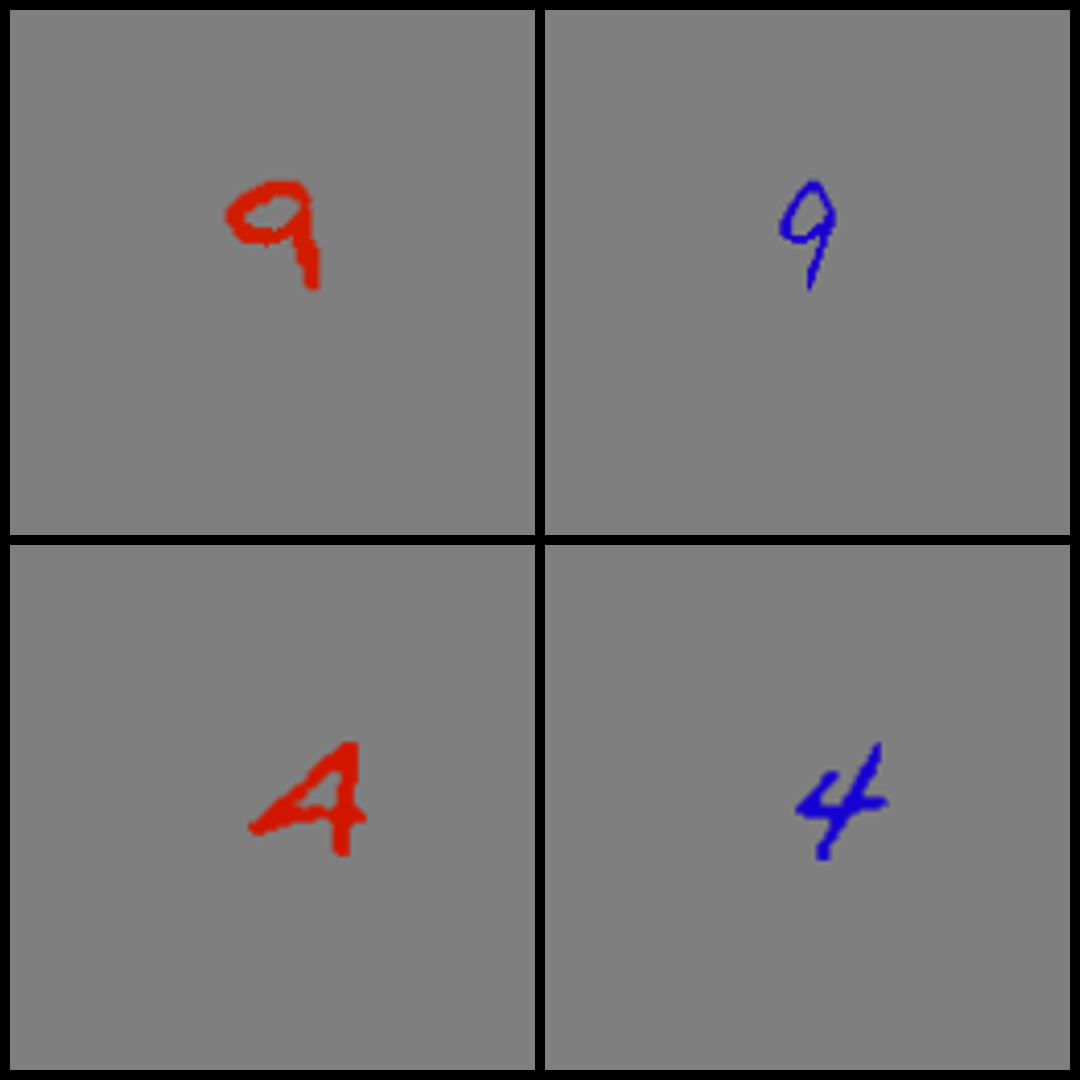
\includegraphics[height=1.8cm]{img/distribution/train_collage.png}
			\caption*{Train}
		\end{subfigure}%
		\hfill
		\begin{subfigure}[b]{0.2\textwidth}
			\centering
			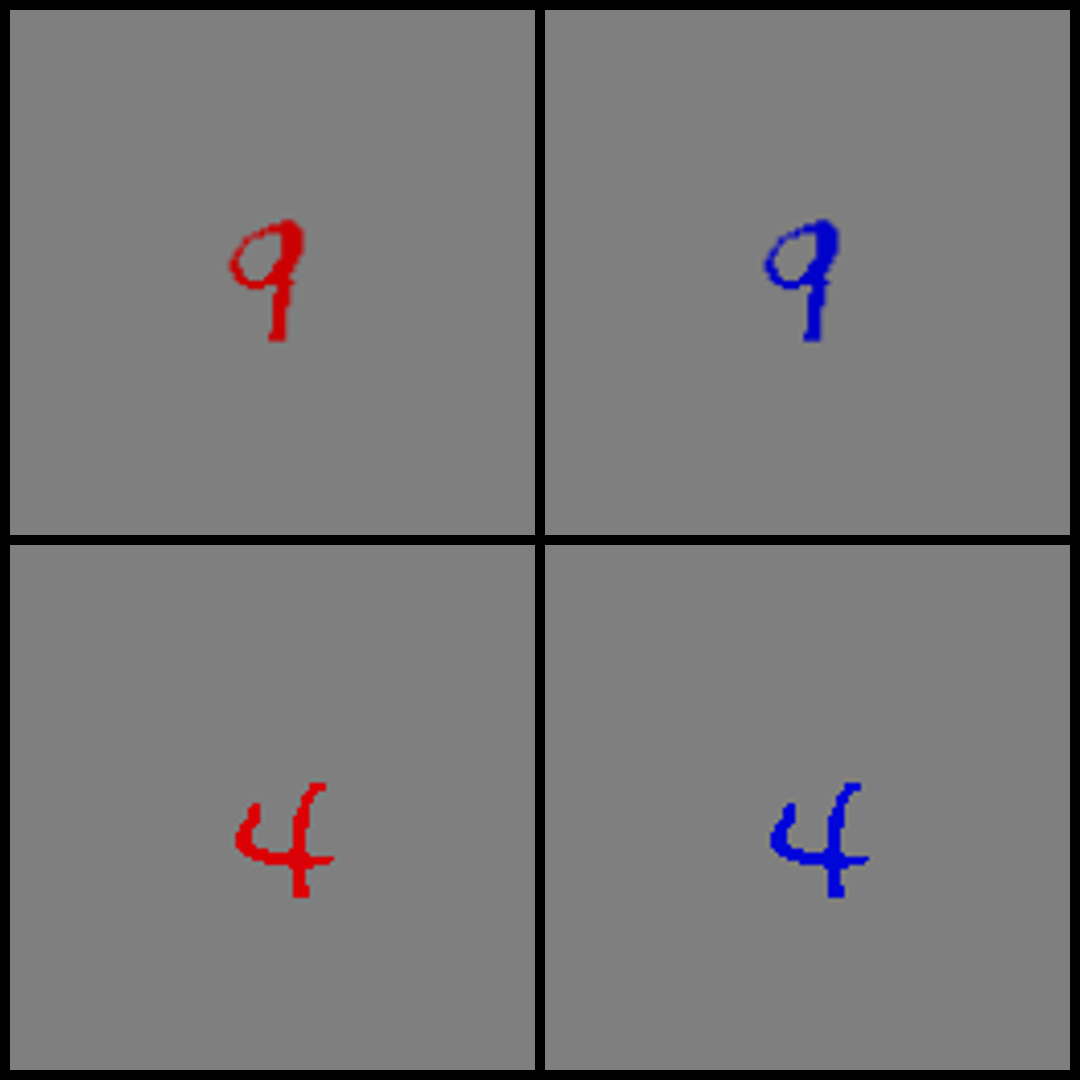
\includegraphics[height=1.8cm]{img/distribution/val_collage.png}
			\caption*{Validation}
		\end{subfigure}%
		\hfill
		\begin{subfigure}[b]{0.6\textwidth}
			\centering
			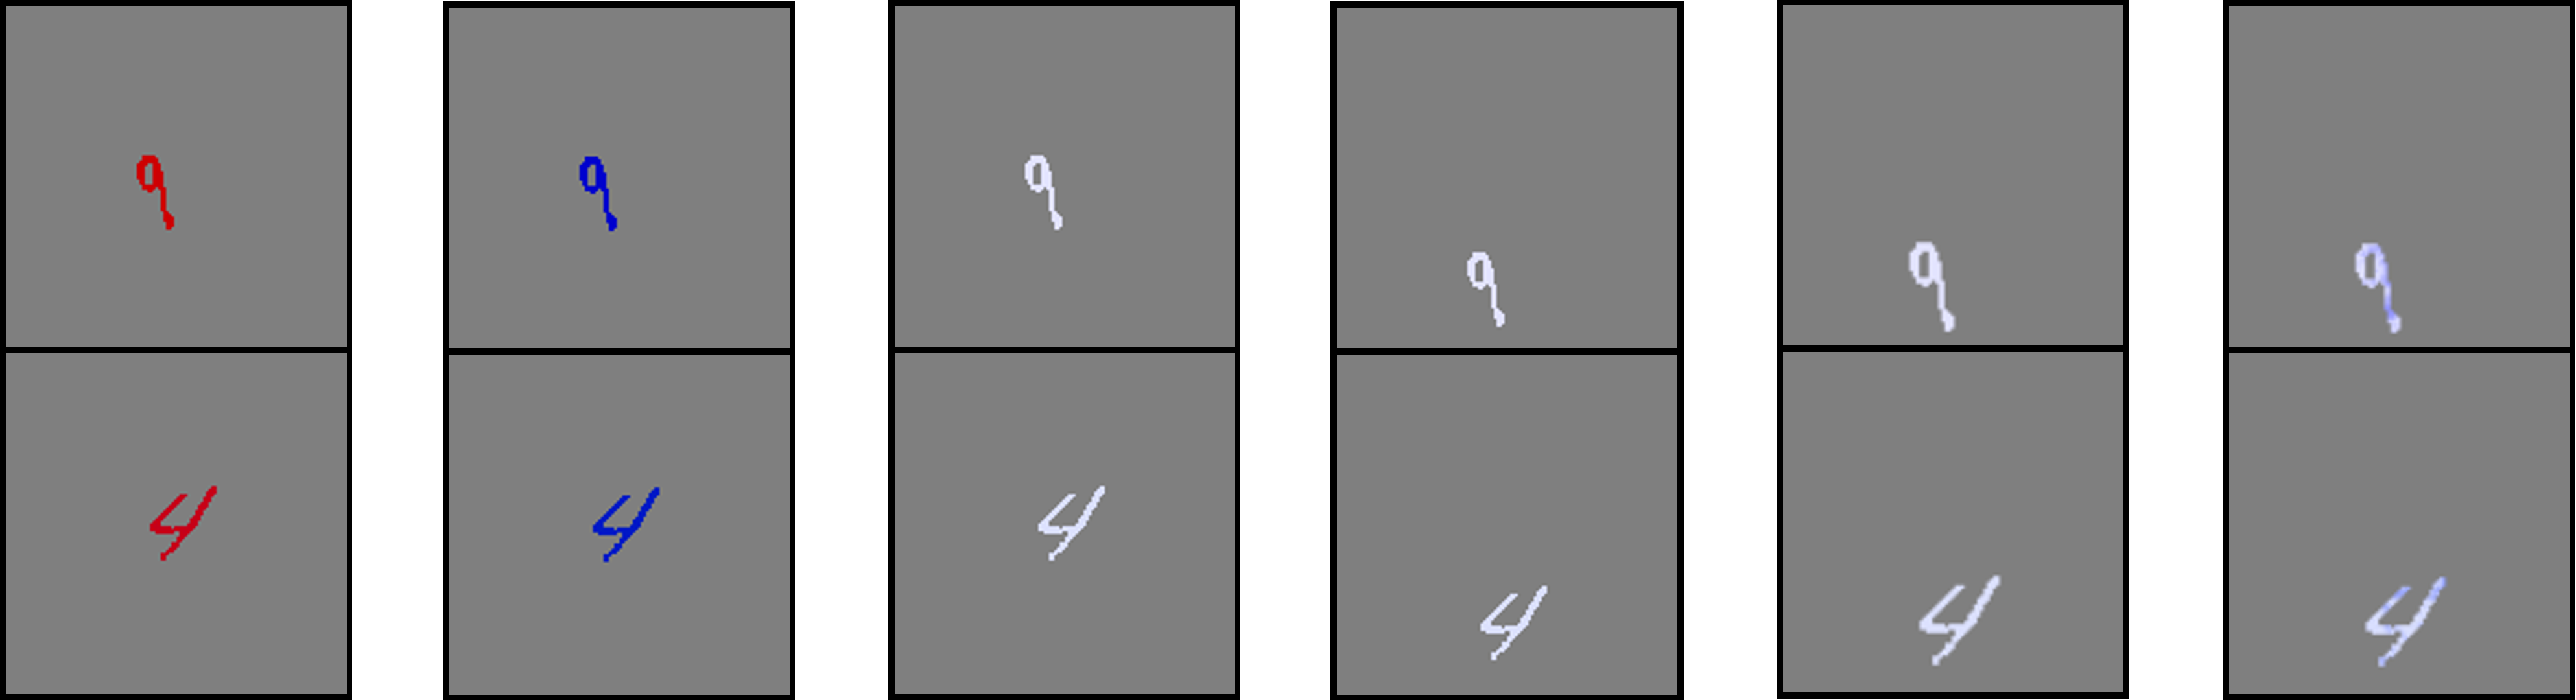
\includegraphics[height=1.8cm]{img/distribution/test_collage2.png}
			\caption*{Test (0 - 5)}
		\end{subfigure}
	\end{figure}

\end{frame}

% \begin{frame}{Out-of-distribution setting -- Paired samples}

% 	\vspace{0.2cm}

% 	\textbf{Experiment 1.} $D^{\text{val}}$ and $D^{\text{test}}$ are each generated from a single MNIST sample.
	
% 	\begin{figure}[H]
% 		\centering
% 		\begin{subfigure}[b]{0.3\textwidth}
% 			\centering
% 			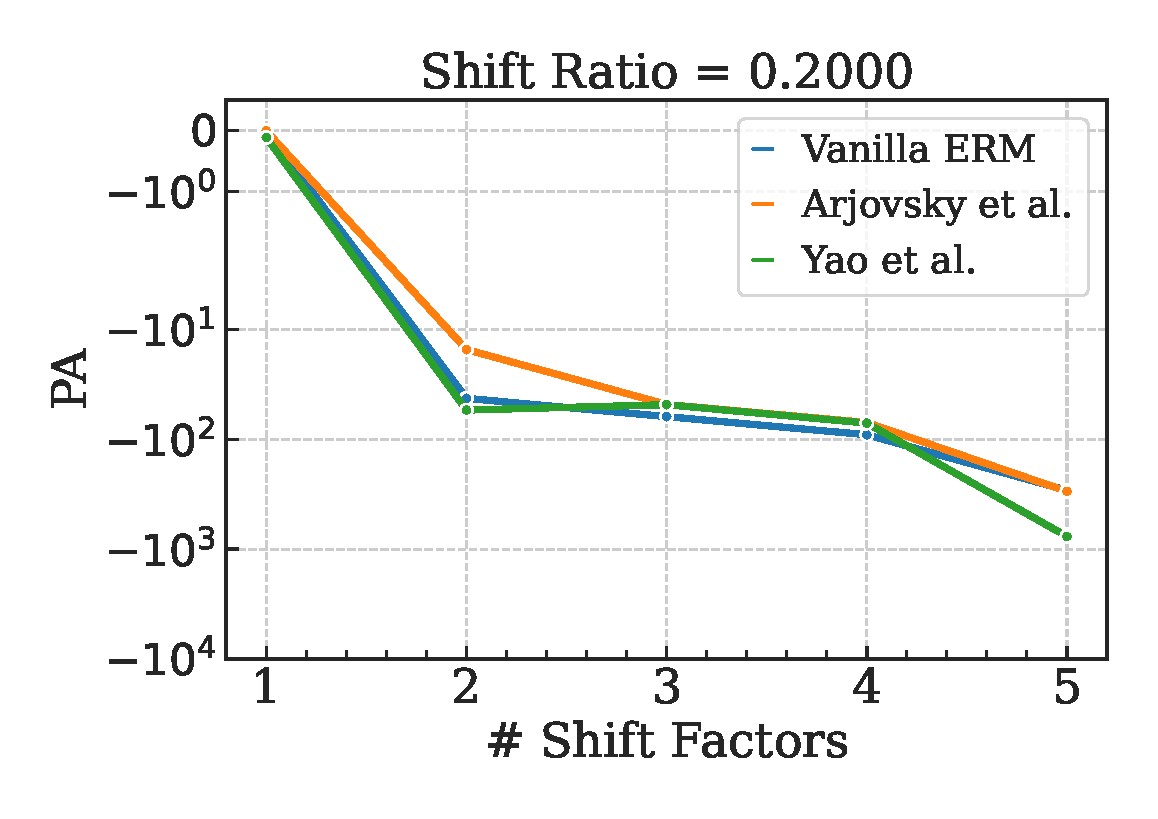
\includegraphics[width=\textwidth]{img/distribution/paper_nonpaired_sel=acc_met=PA_sr=0.2.pdf}
% 		\end{subfigure}
% 		\hfill
% 		\begin{subfigure}[b]{0.3\textwidth}
% 			\centering
% 			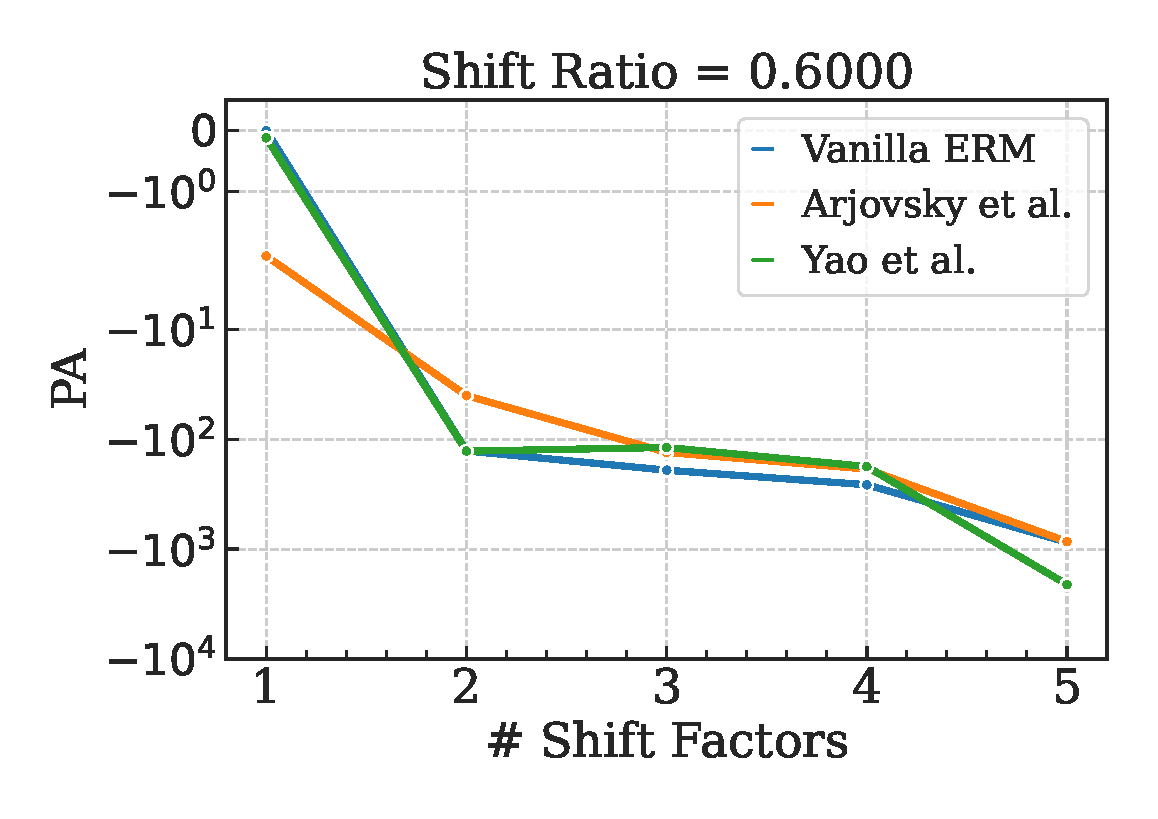
\includegraphics[width=\textwidth]{img/distribution/paper_nonpaired_sel=acc_met=PA_sr=0.6.pdf}
% 		\end{subfigure}
% 		\hfill
% 		\begin{subfigure}[b]{0.3\textwidth}
% 			\centering
% 			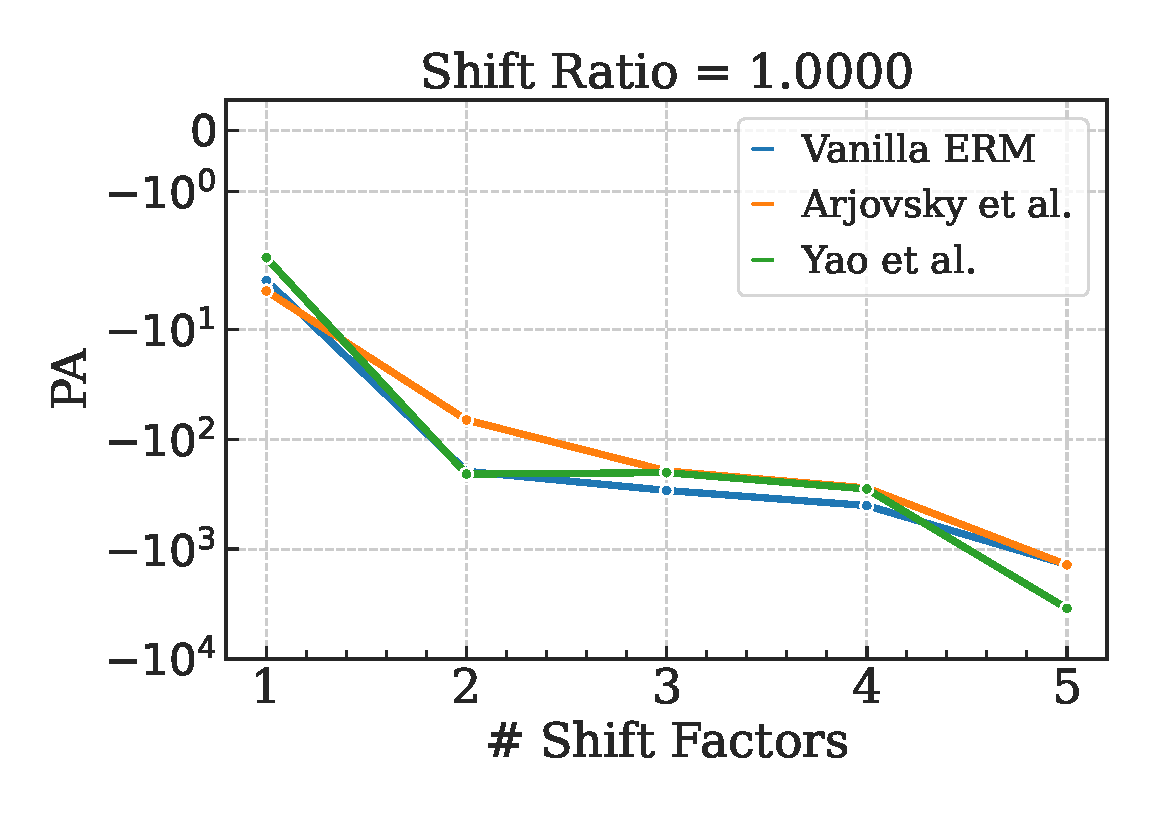
\includegraphics[width=\textwidth]{img/distribution/paper_nonpaired_sel=acc_met=PA_sr=1.0.pdf}
% 		\end{subfigure}
	
% 		\caption{
% 		Evolution of PA under increasing levels of shift power and shift ratio $\alpha$.
% 		}
% 	\end{figure}

% 	\vspace{-0.2cm}
	
% 	\begin{table}[H]
% 		\centering
% 		\resizebox{\textwidth}{!}{%
% 		\begin{tabular}{l|ccc|ccc|ccc|ccc}
% 		\multirow{2}{*}{} & \multicolumn{3}{c|}{1 Shifted Factor} & \multicolumn{3}{c|}{2 Shifted Factors} & \multicolumn{3}{c|}{3 Shifted Factors} & \multicolumn{3}{c}{4 Shifted Factors}\\
% 		 & PA & $\operatorname{AFR}_{\text{P}}$ & $\operatorname{AFR}_{\text{T}}$ & PA & $\operatorname{AFR}_{\text{P}}$  & $\operatorname{AFR}_{\text{T}}$ & PA & $\operatorname{AFR}_{\text{P}}$  & $\operatorname{AFR}_{\text{T}}$ & PA & $\operatorname{AFR}_{\text{P}}$  & $\operatorname{AFR}_{\text{T}}$ \\
% 		\midrule
% 		{\color{tab:blue} \textbf{Vanilla ERM}} & -3.583 & 0.999 & 0.992 & -195.4	& 0.979 & 0.973 & 291.8 & 0.968 & 0.963 & -400.9 & 0.957 & 0.953 \\
% 		{\color{tab:orange} \textbf{Arjovsky et al.}} & -4.463 & 0.999 & 0.989 & \textbf{-66.54} & \textbf{0.994} & 0.987 & \textbf{-194.2} & 0.982 & 0.978 & \textbf{-277.1} & 0.974 & \textbf{0.972} \\
% 		{\color{tab:green} \textbf{Yao et al.}} & \textbf{-2.219} & \textbf{0.999} & \textbf{0.993} & -207.2 & 0.980 & \textbf{0.975} & -200.9 & \textbf{0.983} & \textbf{0.979} & -282.9 & \textbf{0.976} & 0.970 \\
% 		\bottomrule
% 		\end{tabular}
% 		}
% 		\caption{
% 			Comparison of PA, $\operatorname{AFR}_{\text{P}}$ and $\operatorname{AFR}_{\text{T}}$ scores
% 			for $\alpha=1$.
% 		}
% 	\end{table}
% \end{frame}

\begin{frame}{Out-of-distribution setting -- Non-paired samples}

	\vspace{0.2cm}

	\textbf{Experiment 2.} $D^{\text{val}}$ and $D^{\text{test}}$ are each generated from a different MNIST sample.
	
	\begin{figure}[H]
		\centering
		\begin{subfigure}[b]{0.3\textwidth}
			\centering
			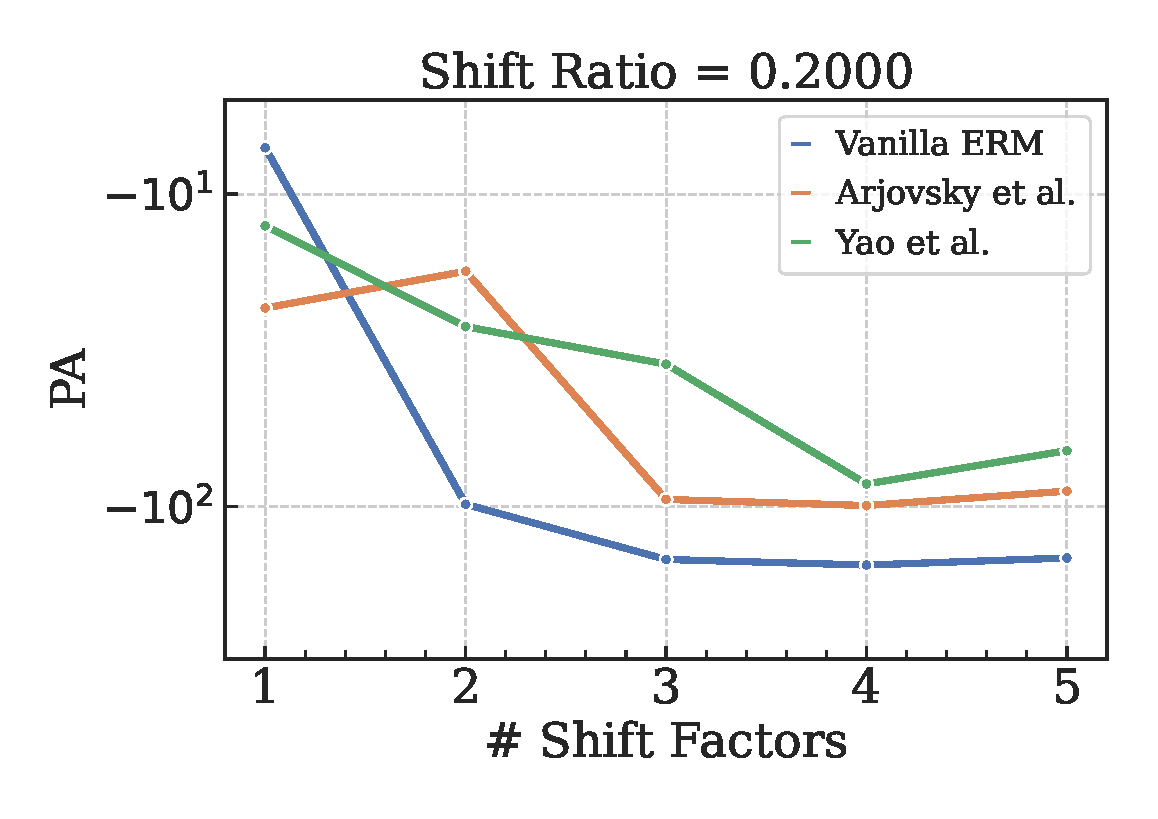
\includegraphics[width=\textwidth]{img/distribution/shift_ratio=0.200.pdf}
		\end{subfigure}
		\hfill
		\begin{subfigure}[b]{0.3\textwidth}
			\centering
			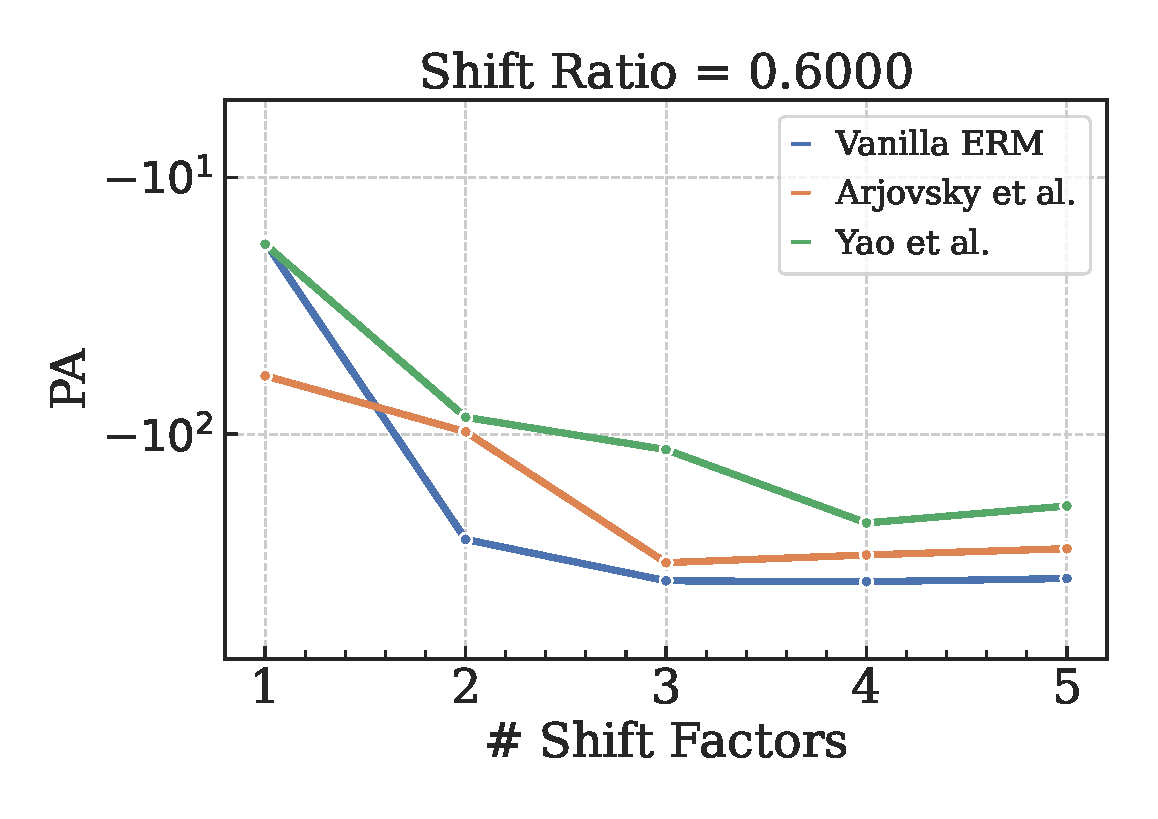
\includegraphics[width=\textwidth]{img/distribution/shift_ratio=0.600.pdf}
		\end{subfigure}
		\hfill
		\begin{subfigure}[b]{0.3\textwidth}
			\centering
			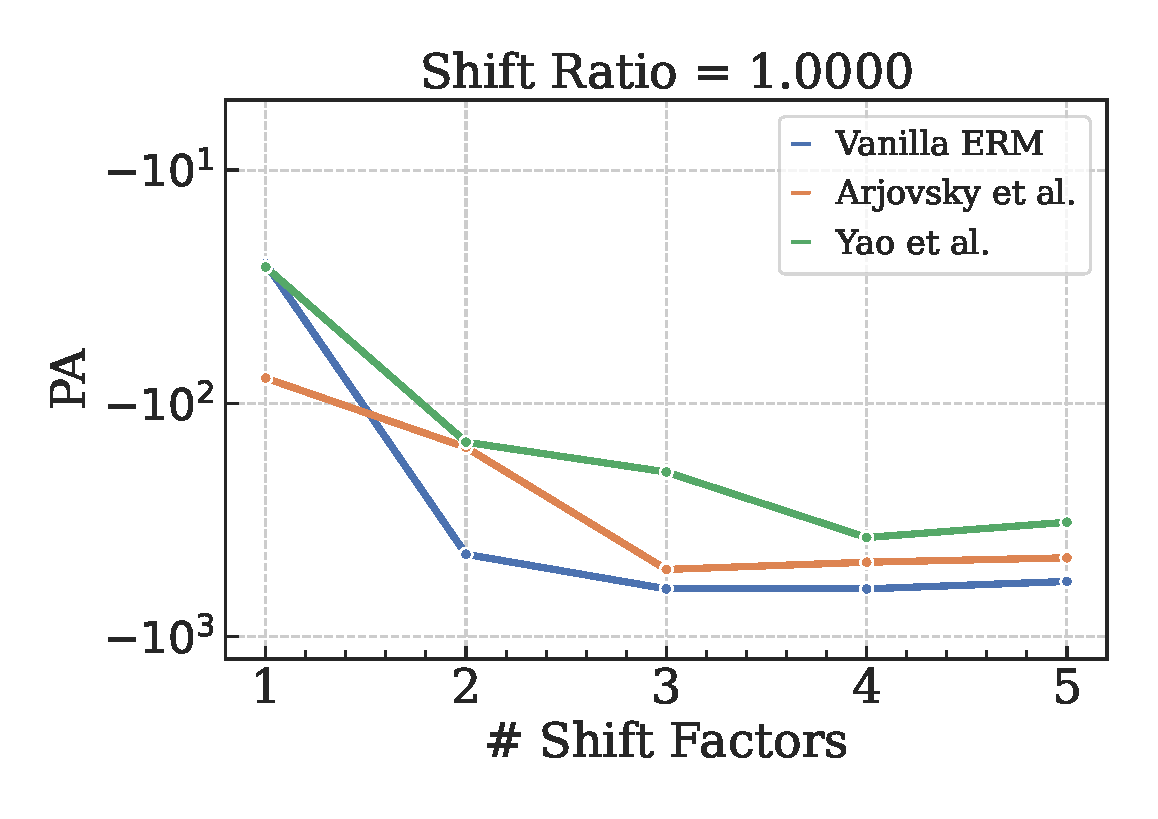
\includegraphics[width=\textwidth]{img/distribution/shift_ratio=1.000.pdf}
		\end{subfigure}
	
		\caption{
		Evolution of PA under increasing levels of shift power and shift ratio $\alpha$.
		}
	\end{figure}

	\vspace{-0.2cm}
	
	\begin{table}[H]
		\centering
		\resizebox{0.8\textwidth}{!}{%
		\begin{tabular}{l|ccc|ccc|ccc}
		\multirow{2}{*}{} & \multicolumn{3}{c|}{1 Shifted Factor} & \multicolumn{3}{c|}{3 Shifted Factors} & \multicolumn{3}{c}{5 Shifted Factors} \\
		& PA & $\operatorname{AFR}_{\text{P}}$ & $\operatorname{AFR}_{\text{T}}$ & PA & $\operatorname{AFR}_{\text{P}}$  & $\operatorname{AFR}_{\text{T}}$ & PA & $\operatorname{AFR}_{\text{P}}$  & $\operatorname{AFR}_{\text{T}}$ \\
		\midrule
		{\color{tab:blue} \textbf{Vanilla ERM}} & \textbf{-24.91}  & 0.999 & 0.993 & -625.6 & 0.979 & 0.975 & -579.4 & 0.976 & 0.873 \\
		{\color{tab:orange} \textbf{Arjovsky et al.}} & -76.76 & 0.998 & 0.993 & -514.2 & 0.976 & 0.978  & -464.2 & 0.976 & 0.911 \\
		{\color{tab:green} \textbf{Yao et al.}} & -26.21 & \textbf{0.999} & \textbf{0.994} & \textbf{-201.2} & \textbf{0.985} & \textbf{0.980} & \textbf{-324.4} & \textbf{0.988} & \textbf{0.945} \\
		\bottomrule
		\end{tabular}
		}
		\caption{
			Comparison of PA, $\operatorname{AFR}_{\text{P}}$ and $\operatorname{AFR}_{\text{T}}$ scores
			for $\alpha=1$.
		}
	\end{table}

\end{frame}


\newsection{Model selection}
\begin{frame}
    \centering
    \Huge{\insertsection}  % This will display the section title
\end{frame}

\begin{frame}{Model selection -- Challenges}
	\begin{itemize}
		\item Agreement between predictive outcomes across different samples no longer
		guarantees that the set of features learned are relevant for the task at hand.
		\item A classifier overfitting to specific features during training would lower
		its performance on validation data and simultaneously be considered robust.
		\item The ultimate measure of domain adaptation capabilities is accuracy
		on target domains.

		\vspace{0.5cm}
		\textbf{Experiment 1.} Access to target domains for model selection purposes is sequentially
		increased. In most cases, $\bm{x}_0^{\text{val}}$ will belong to the source.

		\vspace{0.2cm}
		\textbf{Experiment 2.} The inductive bias of the model is artificially manipulated to
		encode shortcut learning opportunities. 
	\end{itemize}

\end{frame}

\begin{frame}{Model selection -- Experiment 1}
	\textbf{Experimental setup.} Both position and hue are considered as learning factors.

	\begin{table}[H]
        \centering
		\resizebox{0.8\textwidth}{!}{%
        \begin{tabular}{c|c|c|c|c|c|c|c}
             & Env. & Hue & Lightness & Position & Scale & Texture & \textit{Shape} \\
            \specialrule{1.5pt}{1pt}{1pt}  % Thicker line
            \multirow{2}{*}{Training} 
            & 0 & red & dark & CC & large & blank & \textit{1,4,7,9} \\
            & 1 & \textbf{blue} & dark & CC & large & blank & \textit{1,4,7,9} \\
            \specialrule{1.5pt}{1pt}{1pt}  % Thicker line
            \multirow{1}{*}{Validation} 
            & 0 & red & dark & CC & large & blank & \textit{1,4,7,9} \\
            \hline
            \multirow{1}{*}{SD} 
            & 1 & red & dark & CC & large & blank & \textit{1,4,7,9} \\
            \multirow{1}{*}{ID} 
            & 1 & \textbf{blue} & dark & CC & large & blank & \textit{1,4,7,9} \\
            \multirow{1}{*}{1F-MD} 
            & 1 & \textbf{magenta} & dark & CC & large & blank & \textit{1,4,7,9} \\
            \multirow{1}{*}{5F-MD} 
            & 1 & \textbf{green} & \textbf{bright} & \textbf{UL} & \textbf{small} & \textbf{tiles} & \textit{1,4,7,9} \\
            \specialrule{1.5pt}{1pt}{1pt}  % Thicker line
            \multirow{2}{*}{Validation OOD} 
            & 0 & \textbf{yellow} & dark & CC & large & blank & \textit{1,4,7,9} \\
            & 1 & \textbf{magenta} & dark & CC & large & blank & \textit{1,4,7,9} \\
            \specialrule{1.5pt}{1pt}{1pt}  % Thicker line
        \end{tabular}
		}
        \caption{
        Factors associated with each of the environments considered in this experiment (hue). CC and UL account
        for 'centered center' and 'upper left', respectively.
        }
        \label{ds:hue_trainval}
    \end{table}
\end{frame}

\begin{frame}{Model selection -- Experiment 1}
	\begin{table}[H]
		\centering
		\setlength{\tabcolsep}{2.5pt}
		\resizebox{0.8\textwidth}{!}{%
		\begin{tabular}{l|ccc|ccc|ccc|ccc|ccc|ccc}
		\multirow{3}{*}{} & \multicolumn{3}{c|}{\textbf{Acc. Test 0}} & \multicolumn{3}{c|}{\textbf{Acc. Test 1}} & \multicolumn{3}{c|}{\textbf{Acc. Test 2}} & \multicolumn{3}{c|}{\textbf{Acc. Test 3}} & \multicolumn{3}{c|}{\textbf{Acc. Test 4}} & \multicolumn{3}{c}{\textbf{Acc. Test 5}} \\
		\textbf{{\color{tab:orange} \textbf{IRM}}} & Acc. & AFR$_\text{P}$ & PA & Acc. & AFR$_\text{P}$ & PA & Acc. & AFR$_\text{P}$ & PA & Acc. & AFR$_\text{P}$ & PA & Acc. & AFR$_\text{P}$ & PA & Acc. & AFR$_\text{P}$ & PA \\
		\midrule
		SD & 99.3 & 99.3 & 99.3 & 71.5 & 71.5 & {\textbf{83.3}} & 70.6 & 70.6 & {\textbf{91.9}} & 65.3 & 65.3 & {\textbf{85.9}} & {\textbf{75.0}} & \textbf{75.0} & 66.5 & 28.8 & 28.8 & {\textbf{46.7}} \\
		ID & 99.4 & 99.4 & 99.4 & 44.3 & 44.3 & 44.3 & 88.1 & 88.1 & 88.1 & 76.1 & 76.1 & 76.1 & 59.4 & 59.4 & 59.4 & 45.2 & 45.2 & 45.2 \\
		1F-MD & 99.4 & 99.4 & 99.4 & 44.3 & 44.3 & 44.3 & 88.1 & 88.1 & 88.1 & 76.1 & 76.1 & 76.1 & 59.4 & 59.4 & 59.4 & 45.2 & 45.2 & 45.2 \\
		5F-MD & {\textbf{99.4}} & \textbf{99.4} & 99.3 & 31.2 & 31.2 & {\textbf{83.3}} & 88.7 & 88.7 & {\textbf{91.9}} & 73.8 & 73.8 & {\textbf{85.9}} & 65.5 & 65.5 & {\textbf{66.5}} & {\textbf{50.2}} & \textbf{50.2} & 46.7 \\
		OOD & 99.5 & 99.5 & 99.5 & 62.4 & 62.4 & 62.4 & 90.1 & 90.1 & 90.1 & 84.1 & 84.1 & 84.1 & 52.2 & 52.2 & 52.2 & 42.6 & 42.6 & 42.6 \\
		\midrule
		\addlinespace
		\addlinespace
		\textbf{{\color{tab:green} \textbf{LISA}}} & Acc. & AFR$_\text{P}$ & PA & Acc. & AFR$_\text{P}$ & PA & Acc. & AFR$_\text{P}$ & PA & Acc. & AFR$_\text{P}$ & PA & Acc. & AFR$_\text{P}$ & PA & Acc. & AFR$_\text{P}$ & PA \\
		\midrule
		SD & 99.3 & 99.3 & {\textbf{99.4}} & {\textbf{88.4}} & \textbf{88.4} & 83.1 & 53.9 & 53.9 & {\textbf{78.5}} & 57.9 & 57.9 & {\textbf{80.5}} & 63.1 & 63.1 & {\textbf{77.0}} & {\textbf{38.8}} & \textbf{38.8} & 35.4 \\
		ID & 99.5 & 99.5 & 99.5 & 59.2 & 59.2 & {\textbf{88.8}} & {\textbf{62.5}} & \textbf{62.5} & 60.4 & 71.7 & 71.7 & {\textbf{76.8}} & 70.9 & 70.9 & {\textbf{71.5}} & 35.2 & 35.2 & {\textbf{36.4}} \\
		1F-MD & 99.5 & 99.5 & 99.5 & 88.8 & 88.8 & 88.8 & 54.4 & 54.4 & 54.4 & 76.8 & 76.8 & 76.8 & 71.5 & 71.5 & 71.5 & 36.4 & 36.4 & 36.4 \\
		5F-MD & 99.2 & 99.2 & {\textbf{99.4}} & {\textbf{86.6}} & \textbf{86.6} & 85.1 & 71.1 & 71.1 & {\textbf{74.8}} & 77.3 & 77.3 & {\textbf{83.7}} & 73.7 & 73.7 & {\textbf{81.9}} & {\textbf{49.4}} & \textbf{49.4} & 48.6 \\
		OOD & {\textbf{99.3}} & 99.2 & 99.2 & 91.8 & {\textbf{95.8}} & 84.4 & 59.0 & 63.0 & {\textbf{83.0}} & 77.6 & 79.0 & {\textbf{88.0}} & 73.8 & 73.6 & {\textbf{84.8}} & 34.4 & 40.4 & {\textbf{47.3}} \\
		\bottomrule
	\end{tabular}%
	}
	\caption{
		Test performance under increasing levels of shift for models selected through different configurations of 
		validation datasets. PA, AFR$_{\text{P}}$ and accuracy are used as early stopping criteria for model selection
		in the hue factor experiment.}
	\end{table}
\end{frame}

\begin{frame}{Model selection -- Experiment 2}
	\textbf{Experimental setup.} Both position and hue are considered as learning factors.

	% \begin{itemize}
    %     \item Zero generalization opportunities (ZGO): Each instance of $F^P$ is exclusively co-occurrent with a 
    %     unique instance of $F^L$. The model is expected to overfit to spurious correlations and thus generalize
    %     poorly to datasets in which these are not present.
    %     \item Compositional generalization opportunities (CGO): Starting from the ZGO setting, the exclusive co-occurrence
    %     between some instances of $F^P$ and $F^L$ is broken by the presence of generalization opportunities. The model 
    %     should be increasingly robust to unseen combinations the higher is the number of generalization opportunities.
    %     \item Zero shortcut opportunities (ZSO): All instances of $F^P$ are uniformly co-occurrent with all 
    %     instances of $F^L$, so that all combinations of factors are present in source domains.
    % \end{itemize}

    The setting for ID model selection (i.e. domain adaptation) requires that validation datasets contain the
    same configuration of factors than the training datasets. Experiments will be performed for
    ZGO, ZSO and single, double and triple CGO.

    \begin{figure}[H]
        \centering
        % LEGEND
        \begin{subfigure}[b]{\textwidth}
            \centering
            % Here, you would include your legend, for example, a dummy image
            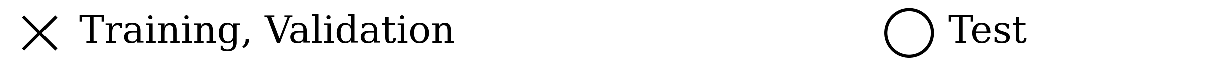
\includegraphics[width=0.6\textwidth]{img/msel/_legend_theory.pdf}
        \end{subfigure}
        \vspace{-0.2cm} % Add some vertical space between the legend and the subfigures

        \begin{subfigure}[b]{0.17\textwidth}
            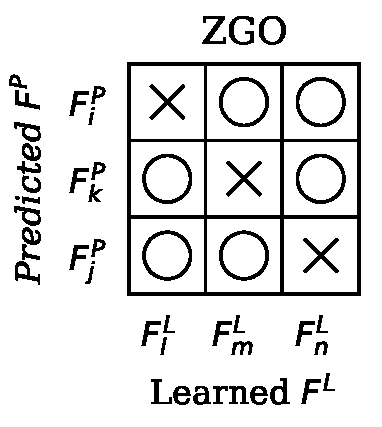
\includegraphics[width=\textwidth]{img/msel/_ZGO.pdf}
        \end{subfigure}
        \hfill
        \begin{subfigure}[b]{0.17\textwidth}
            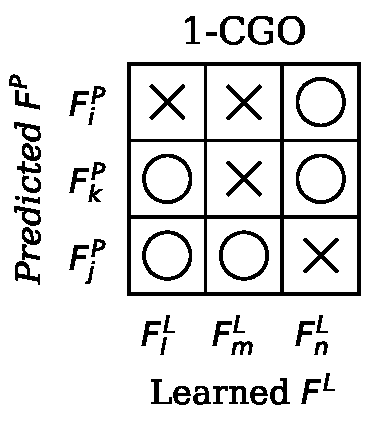
\includegraphics[width=\textwidth]{img/msel/_1-CGO.pdf}
        \end{subfigure}
        \hfill
        \begin{subfigure}[b]{0.17\textwidth}
            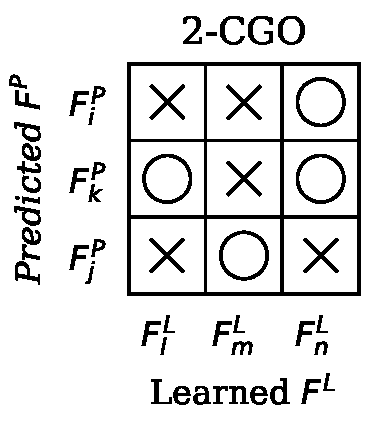
\includegraphics[width=\textwidth]{img/msel/_2-CGO.pdf}
        \end{subfigure}
        \hfill
        \begin{subfigure}[b]{0.17\textwidth}
            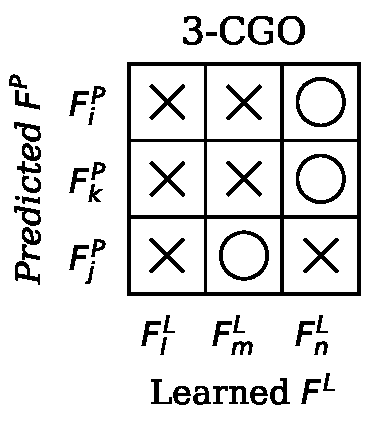
\includegraphics[width=\textwidth]{img/msel/_3-CGO.pdf}
        \end{subfigure}
        \hfill
        \begin{subfigure}[b]{0.17\textwidth}
            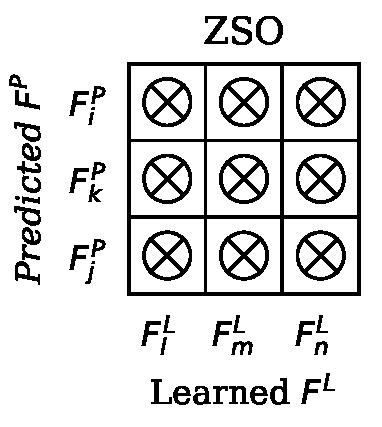
\includegraphics[width=\textwidth]{img/msel/_ZSO.pdf}
        \end{subfigure}
        
        \caption{Representation of the co-occurrence pattern in between learning factors $F^L$ and predicted
        factors $F^P$ for the ZGO, CGO and ZSO settings that will be considered in this experiment.
        }
    \end{figure}

\end{frame}
	
\begin{frame}{Model selection -- Experiment 2}
	\begin{table}[H]
		\centering
		\resizebox{0.7\textwidth}{!}{%
		\begin{tabular}{l|cl|cl|cl|cl|cl}
		\multirow{2}{*}{} & \multicolumn{2}{c|}{\textbf{Test 1}} & \multicolumn{2}{c|}{\textbf{Test 2}} & \multicolumn{2}{c|}{\textbf{Test 3}} & \multicolumn{2}{c|}{\textbf{Test 4}} & \multicolumn{2}{c}{\textbf{Test 5}} \\
		\textbf{{\color{tab:blue} \textbf{ERM}}} & Acc. & $\Delta$Acc. & Acc. & $\Delta$Acc. & Acc. & $\Delta$Acc. & Acc. & $\Delta$Acc. & Acc. & $\Delta$Acc. \\
		\midrule
		ZGO & 53.2 & \PlusMinus 0.01 & 54.6 & \PlusMinus 0.01 & 55.7 & \PlusMinus 0.01 & 66.7 & \PlusMinus 0.01 & 66.6 & \PlusMinus 0.01 \\
		1-CGO & 62.9 & {\color{tab:green}  \textbf{\Plus 9.5}} & 64.7 & {\color{tab:green}  \textbf{\Plus 10.2}} & 60.8 & {\color{tab:green}  \textbf{\Plus 0.3}} & 62.9 & {\color{tab:green}  \textbf{\Plus 2.2}} & 64.2 & {\color{tab:green}  \textbf{\Plus 0.5}} \\
		2-CGO & 69.1 & {\color{tab:green}  \textbf{\Plus 9.4}} & 71.2 & {\color{tab:green}  \textbf{\Plus 7.8}} & 71.9 & {\color{tab:green}  \textbf{\Plus 0.3}} & 76.2 & {\color{tab:red} \textbf{\Minus 2.4}} & 77.0 & {\color{tab:red} \textbf{\Minus 2.8}} \\
		3-CGO & 73.1 & {\color{tab:green}  \textbf{\Plus 16.6}} & 85.6 & {\color{tab:green}  \textbf{\Plus 3.6}} & 70.1 & {\color{tab:green}  \textbf{\Plus 9.7}} & 71.4 & {\color{tab:green}  \textbf{\Plus 6.4}} & 72.1 & {\color{tab:green}  \textbf{\Plus 6.7}} \\
		ZSO & 99.6 & \PlusMinus 0.01 & 92.8 & {\color{tab:red} \textbf{\Minus 0.1}} & 89.9 & {\color{tab:green}  \textbf{\Plus 0.2}} & 85.9 & \PlusMinus 0.01 & 85.9 & \PlusMinus 0.01 \\
		\midrule
		\addlinespace
		\addlinespace
		\textbf{{\color{tab:orange} \textbf{IRM}}} & Acc. & $\Delta$Acc. & Acc. & $\Delta$Acc. & Acc. & $\Delta$Acc. & Acc. & $\Delta$Acc. & Acc. & $\Delta$Acc. \\
		\midrule
		ZGO & 50.1 & {\color{tab:green}  \textbf{\Plus 5.9}} & 50.5 & {\color{tab:green}  \textbf{\Plus 4.9}} & 52.8 & {\color{tab:green}  \textbf{\Plus 9.5}} & 64.4 & {\color{tab:green}  \textbf{\Plus 1.1}} & 64.9 & {\color{tab:green}  \textbf{\Plus 1.2}} \\
		1-CGO & 63.0 & {\color{tab:green}  \textbf{\Plus 7.0}} & 65.9 & {\color{tab:green}  \textbf{\Plus 7.6}} & 59.4 & {\color{tab:green}  \textbf{\Plus 2.2}} & 60.1 & {\color{tab:green}  \textbf{\Plus 2.2}} & 59.0 & {\color{tab:green}  \textbf{\Plus 1.8}} \\
		2-CGO & 69.0 & {\color{tab:green}  \textbf{\Plus 10.6}} & 69.7 & {\color{tab:green}  \textbf{\Plus 10.0}} & 67.5 & {\color{tab:green}  \textbf{\Plus 4.7}} & 64.5 & {\color{tab:green}  \textbf{\Plus 13.0}} & 65.1 & {\color{tab:green}  \textbf{\Plus 12.6}} \\
		3-CGO & 79.5 & {\color{tab:green}  \textbf{\Plus 11.6}} & 83.0 & {\color{tab:green}  \textbf{\Plus 9.8}} & 73.6 & {\color{tab:green}  \textbf{\Plus 10.9}} & 70.7 & {\color{tab:green}  \textbf{\Plus 11.0}} & 72.2 & {\color{tab:green}  \textbf{\Plus 11.3}} \\
		ZSO & 99.4 & {\color{tab:green}  \textbf{\Plus 0.1}} & 93.4 & {\color{tab:green}  \textbf{\Plus 1.3}} & 89.2 & {\color{tab:green}  \textbf{\Plus 0.2}} & 87.0 & {\color{tab:green}  \textbf{\Plus 1.6}} & 87.0 & {\color{tab:green}  \textbf{\Plus 1.6}} \\
		\bottomrule
		\end{tabular}%
		}
		\caption{
			Test performance under increasing levels of shift for models selected through different configurations of factor
			co-occurrence for the hue learning factor experiment. Specifically, the performance of models selected through validation accuracy (Acc) and
			the difference between accuracy-based and PA-based selection ($\Delta$Acc) is reported.
		}
		\label{tab:sogo_hue_improve}
	\end{table}
\end{frame}

\newsection{Domain adaptation in WILDS}
\begin{frame}
    \centering
    \Huge{\insertsection}  % This will display the section title
\end{frame}

\begin{frame}{WILDS -- Dataset 1}
	\textbf{Experiment 1.} The \textbf{waterbirds} dataset was considered. The classes \texttt{waterbird} and
	\texttt{landbird} are influenced by a spurious correlation with the background.
	\begin{table}[H]
		\centering
		\resizebox{0.5\textwidth}{!}{%
		\begin{tabular}{l|c|c|c}
		& Training & Validation & Test \\
		\midrule
		Ratio water / land & $\sim 2.86$  & $\sim 1$ & $\sim 1$ \\
		\bottomrule
		\end{tabular}
		}
	\end{table}

	\vspace{0.8cm}

	\begin{table}[H]
		\centering
		\resizebox{0.4\textwidth}{!}{%
		\setlength{\tabcolsep}{2.5pt}
		\begin{tabular}{l|ccc|ccc}
		\multirow{3}{*}{} & \multicolumn{3}{c|}{\textbf{Average Acc.}} & \multicolumn{3}{c}{\textbf{Worst-case Acc.}}\\
		& Acc. & AFR$_\text{P}$ & PA & Acc. & AFR$_\text{P}$ & PA \\
		\midrule
		\textbf{{\color{tab:blue} \textbf{ERM}}} & \textbf{78.52} & 73.72 & \textbf{78.52} & \textbf{67.11} & 58.90 & \textbf{67.11} \\
		\textbf{{\color{tab:orange} \textbf{IRM}}} & \textbf{90.16} & 89.70 & \textbf{90.16} & \textbf{89.21} & 88.67 & \textbf{89.21} \\
		\bottomrule
		\end{tabular}
		}
		\caption{
			Average and worst-case test accuracy for the \texttt{waterbirds} \cite{kohWILDSBenchmarkIntheWild2021} dataset.
		}
		\label{tab:waterbirds}
	\end{table}
\end{frame}

\begin{frame}{WILDS -- Dataset 2}
	\textbf{Experiment 2.} The \textbf{celebA} dataset was considered. The classification task involves the
	prediction of hair color from images of American celebrities. The subpopulation shift arises from the spurious correlation 
	with the gender.

	\begin{table}[H]
		\centering
		\resizebox{0.32\textwidth}{!}{%
		\begin{tabular}{l|c|c}
		& \texttt{blonde} & \texttt{not blonde} \\
		\midrule
		Male   & 1741   & 89931  \\
		Female & 28234   & 82685   \\
		\bottomrule
		\end{tabular}
		}
	\end{table}

	\vspace{0.8cm}

	\begin{table}[H]
		\centering
		\resizebox{0.4\textwidth}{!}{%
		\setlength{\tabcolsep}{2.5pt}
		\begin{tabular}{l|ccc|ccc}
		\multirow{3}{*}{} & \multicolumn{3}{c|}{\textbf{Average Acc.}} & \multicolumn{3}{c}{\textbf{Worst-case Acc.}}\\
		 & Acc. & AFR$_\text{P}$ & PA & Acc. & AFR$_\text{P}$ & PA \\
		\midrule
		\textbf{{\color{tab:blue} \textbf{ERM}}} & 97.80 & \textbf{98.27} & \textbf{98.27} & 97.76 & \textbf{97.77} & \textbf{97.77}\\
		\textbf{{\color{tab:orange} \textbf{IRM}}} & 98.12 & \textbf{98.41} & \textbf{98.41} & \textbf{98.06} & 98.05 & 98.05 \\
		\bottomrule
		\end{tabular}
		}
		\caption{
			Average and worst-case test accuracy for the \texttt{celebA} \cite{kohWILDSBenchmarkIntheWild2021} dataset.
		}
	\end{table}
\end{frame}

\begin{frame}{WILDS -- Dataset 3}
	\textbf{Experiment 3.} The \textbf{camelyon17} dataset was considered. The classification task involves
	the identification of tumor tissue in lymph node patches sampled from different hospitals. The out-of-distribution 
	setting originates from the differences in the samples taken from different hospitals.

	\begin{table}[H]
		\centering
		\resizebox{0.4\textwidth}{!}{%
		\begin{tabular}{l|c|c|c|c}
		Hospital & 1 & 2 & 3 & 4 \\
		\midrule
		Training   & 53425 & 116959 & 132052 & - \\
		Validation & 6011  & 12879  & 14670 & -\\
		Test & - & - & - & 85054 \\
		\bottomrule
		\end{tabular}
		}
	\end{table}

	\begin{table}[H]
		\centering
		\resizebox{0.23\textwidth}{!}{%
		\setlength{\tabcolsep}{2.5pt}
		\begin{tabular}{l|ccc}
		\multirow{3}{*}{} & \multicolumn{3}{c}{\textbf{Accuracy}} \\
		 & Acc. & AFR$_\text{P}$ & PA \\
		\midrule
		\textbf{{\color{tab:blue} \textbf{ERM}}} & 86.73 & 86.73 & 86.73 \\
		\textbf{{\color{tab:orange} \textbf{IRM}}} & 67.98 & 67.98 & 67.98 \\
		\textbf{{\color{tab:green} \textbf{LISA}}} & 81.1 & \textbf{81.8} & \textbf{81.8} \\
		\bottomrule
		\end{tabular}
		}
		\caption{
			Test accuracy for the \texttt{camelyon17} \cite{kohWILDSBenchmarkIntheWild2021} dataset.
		}
		\end{table}
\end{frame}

\newsection{Conclusions}
\begin{frame}
    \centering
    \Huge{\insertsection}  % This will display the section title
\end{frame}

\begin{frame}{Conclusions}
\end{frame}

\newsection{Blibliography}
\begin{frame}
    \centering
    \Huge{\insertsection}  % This will display the section title
\end{frame}

\bibliographystyle{plainnat}
\bibliography{bibliography}
\end{document}


